\svnInfo $Id: raytracing.tex 75 2008-04-07 13:37:13Z axel $
\chapter{Das Raytracingverfahren}
\label{chap:rt}
Seit Beginn der Computergrafik ist eines der Hauptziele die Erzeugung fotorealistischer 2D-Bilder aus einer abstrakten 3D-Beschreibung einer (realen) Szene.Die erzeugten Bilder sollen von Photos nicht zu unterscheiden sein.

Um ein 2D-Bild einer 3D-Szene am Computer anzuzeigen muss die Bildebene in diskrete Bildelemente - die Pixel - aufgeteilt werden. Für jedes Pixel muss zunächst festgestellt werden, welches Objekt ``durch'' dieses Pixel sichtbar ist.
Durch die Eigenschaften des Objekts kann darauf geschlossen werden, wieviel von dem beim Objekt eintreffenden Licht vom betrachteten Punkt auf dem Objekt, in Richtung des Betrachters reflektiert wird.


\section{Rekursives Raytracing}

Beim Raytracing werden zunächst so genannte \textit{Primärstrahlen} generiert: Für jedes Pixel in der Bildebene wird ein Strahl generiert, der bei der Kameraposition entspringt und durch das jeweilige Pixel verläuft. Um den Farbwert des Pixels zu bestimmen wird als nächstes festgestellt welches Objekt der Szene der Strahl in seinem Verlauf als erstes schneidet. Dieser Teil des Raytracings heißt \textbf{Raycasting} und wurde bereits von \cite{Appel68} vorgestellt. Ein Strahl lässt sich mathematisch wie in Gleichung \ref{eq:raysegment} beschreiben. Sind $t_{min} = 0$ und $t_{max} = \infty$ handelt es sich um einen unbegrenzten Strahl, andernfalls um ein Strahlsegment.
Um bestimmen zu können wieviel Licht am Schnittpunkt in die entgegengesetzte Richtung des Strahls abgestrahlt wird, muss jedoch vorher bekannt sein wieviel Licht am Schnittpunkt eintrifft. Danach kann aus den Materialeigenschaften und der Beleuchtung am Schnittpunkt der entsprechende Beitrag zur Intensität des Pixels berechnet werden.

\begin{equation} 
  R = \vec{o_R} + t * \vec{d_R},
  (t \in R, t_{min} <= t < t_{max})
\label{eq:raysegment}
\end{equation}

Den Hauptteil zur Beleuchtung eines Punktes trägt meistens das Licht bei, welches direkt von einer Lichtquelle auf den Punkt abgegeben wird. Wieviel Licht einer Lichtquelle einen Punkt im Raum erreicht hängt zum einen von den Parametern der Lichtquelle ab, aber ebenso von der umliegenden Geometrie, zum Beispiel ob sich ein anderes Objekt zwischen diesem Punkt und der Lichtquelle befindet. Um dies festzustellen werden so genannte \textit{Schattenstrahlen}, die von dem Schnittpunkt zu den Lichtquellen führen, auf Schnitt mit den anderen Objekten der Szene getestet. Wird kein Schnitt gefunden trägt der entsprechende Anteil der Lichtquelle zur Beleuchtung des Schnittpunktes bei.
Für transparente und spiegelnde Materialien beschreibt \cite{Whitted80} die Verfolgung weiterer, so genannter \textit{Sekundärstrahlen}, da das menschliche Auge für diese Phänomene besonders empfindlich ist. Für spiegelnde Materialien wird der ideal reflektierte Strahl nach Gleichung \ref{eq:reflect} berechnet. Für transparente Materialen wird der ideal transmittierte Strahl unter Berücksichtigung des Snelliuschen Brechunggesetzes(Gleichung \ref{eq:refract}) ermittelt. \srcref{core}{vec3}{refract}

Das abgestrahlte Licht an den Schnittpunkten dieser Strahlen trägt ebenfalls zur Beleuchtung des aktuellen Schnittpunkts bei.
Hierfür muss zunächst bestimmt werden, welche Objekte die  \textit{Sekundärstrahlen} treffen und wieviel Licht in Richtung des Schnittpunktes ausgesendet wird. Da es sich hierbei um die selbe Fragestellung wie für den Primärstrahl handelt, lässt sich die Lösung besonders effizient durch Rekursion umsetzen, was dem Verfahren seinen Namen gab.
Durch die Materialeigenschaften des Objekts, auf dem sich der Schnittpunkt befindet wird bestimmt, wieviel von den berechneten Anteilen der Beleuchtung zur Intensität des Pixels beitragen.

\begin{equation}
\label{eq:reflect}
d_{reflect} = \vec{d_r} - 2 * ( \vec{n}_{s} * \vec{d_R} ) * \vec{n}_{s}, |\vec{d_R}| = 1, |\vec{n}_{s}| = 1
\end{equation}
\begin{equation} 
\label{eq:refract}
d_{refract} = ( d_R - ( \vec{n}_{s} * ( \vec{n}_{s} * \vec{d_R} )  ) * \frac{n_{out}}{n_{in}}  - \vec{n}_{s} * \sqrt{( 1 - (\frac{n_{out}}{n_{in}} )^2  * ( 1 - ( \vec{n}_{s} * \vec{d_R} )^2 )}
\end{equation}


\section{Distributed Raytracing}
\begin{figure}
\includegraphics[width=1.0\textwidth]{images/alias.png}
\caption[Unterdrückung von Aliasing-Effekten durch Oversampling]{links: Aliasing beim Rendern ohne Oversampling, rechts: Antialiasing durch Oversampling führt zu glatteren Kanten und Motionblur bei sich bewegenden Objekten}
\label{fig:aliasing}
\end{figure}

Bei der Ermittlung der Farbe eines Pixels durch einen Strahl nimmt man implizit an, dass die Fläche des Pixels unendlich klein ist. Diese Näherung kann zu unerwünschten Aliasingeffekten, wie den bekannten Treppeneffekten (siehe Abbildung \ref{fig:aliasing} links), führen.
Durch \textit{Oversampling} (auch Supersampling) können diese Effekte verringert werden. Das heißt für die Fläche, die der Pixel in der Bildebene verdeckt, werden mehrere Strahlen verfolgt und die Ergebnisse gemittelt.
Das Antialiasing muss sich hierbei nicht nur auf den Bildraum beziehen, sondern kann gleichzeitig auch Bewegungen oder ein virtuelles Kameraobjektiv abtasten. Dieses Verfahren bezeichnet man als \textit{Distributed Raytracing}. Es wurde von \cite{COOK84} entwickelt und ermöglicht die Darstellung von Tiefenschärfe, Bewegungsunschärfe und unscharfen Reflexionen und Schatten. Die Steigerung der Bildqualität geht allerdings mit einem erhöhten Rechenaufwand für die zusätzlichen Strahlen einher.

\section{Global Illumination}


\begin{figure}\center
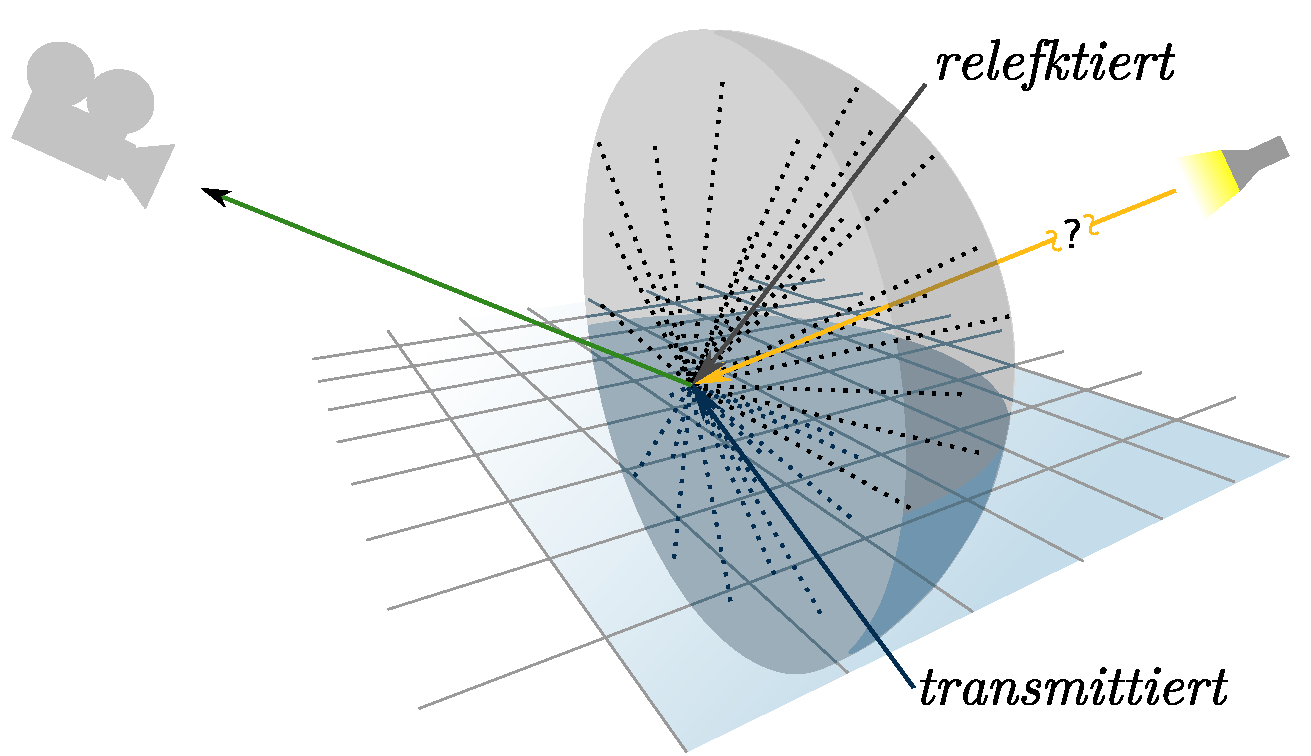
\includegraphics[width=.6\textwidth]{images/refrareflect.pdf}
\caption[Auswahl der Beleuchtungsfaktoren]{Beim Raytracing nach Whitted werden neben den direkten Beleuchtungsanteilen der Lichtquellen ausschließlich der am Schnittpunkt ideal reflektierte sowie der ideal transmittierte Strahl für die Beleuchtung berücksichtigt. Alle weiteren einfallenden Lichtanteile werden ignoriert.}
\label{fig:whitted}
\end{figure}

In der Realität empfängt ein Punkt im Raum aus unendlich vielen Richtungen Licht. Beim Raytracing, wie bisher beschrieben, werden zur Berechnung der Beleuchtung eines Punktes aber nur sehr wenige, ausgewählte Richtungen betrachtet, nämlich die ideal reflektierte, die ideal transmittierte und die Richtungen zu den Lichtquellen (siehe Abbildung \ref{fig:whitted}. Beleuchtung aus anderen Richtungen wird ignoriert. Durch \textit{Distributed Raytracing} können auch unscharfe Reflexionen und Transmissionen dargestellt werden. Der Einfluss von diffuser Reflexion und Bündelung von Licht durch Objekte in der Szene bleibt aber auch hier unbeachtet.
Durch stochastische Emission weiterer Strahlen vom betrachteten Punkt aus, kann eine genauere Abschätzung der Beleuchtung dieses Punktes getroffen werden. Dadurch werden Phänomene wie \textit{Color bleeding} (durch diffuse Reflexion) und \textit{Caustics} (Lichtbündelungseffekte) sichtbar gemacht (siehe Abbildung \ref{fig:gi}. Auch hier resultiert die Steigerung der visuellen Qualität in erhöhtem Rechenaufwand für weitere Strahlberechnungen.

Ein weiteres Phänomen, welches nicht vom klassischen Raytracing dargestellt werden kann, entsteht durch Materialien, die Teile des Lichts weder reflektieren noch \textit{ideal} transmittieren (und es nicht einfach absorbieren). Bei den besagten Materialien tritt das Licht in das Medium ein, wird unter der Oberfläche gestreut und tritt an einer anderen Stelle wieder aus. Marmor ist zum Beispiel ein solches Material, bei dem das so genannte \textit{Subsurface scattering} auftritt.
\begin{figure}
\begin{center}
\includegraphics[width=.6\textwidth]{images/gi.png}

\caption[Globale Beleuchtungsphänomene(Color bleeding, Caustics)]{Die rote Kugel 'blutet' ihre Farbe aus. Dadurch das die Glaskugel das Licht bündelt erscheint die Fläche darunter heller als das Umfeld. \footnotesize{(Erstellt mit dem GI-Raytracer von Mathias Leonhardt)}}
\label{fig:gi}\end{center}
\end{figure}

\section{Problemstellungen}

Alle der genannten Verfahren müssen zur Ermittlung bestimmter Werte Informationen über Schnitte von Strahlen mit der Szene besitzen. Allgemein gilt: je realistischer die Darstellung sein soll, desto mehr Strahlen werden benötigt. Die beschränkt sich nicht nur auf Primärstrahlen.
Doch selbst beim rekursiven Raytracing wird ohne Optimierungen, wie bereits \cite{Whitted80} feststellte, über 90\% der Laufzeit mit der Ermittlung von Strahl-Geometrie-Schnittpunkten verbracht. Die Optimierung der Lösung dieses Problems verspricht demnach den größten Leistungszuwachs für einen Raytracer. 

Die Schnittpunktsuche lässt sich in drei Spezialfälle einteilen:
\begin{description}
       \item[Sichtbarkeit eines Paares von Punkten] Bei diesem Problem handelt es sich um ein Entscheidungsproblem. Es wird danach gefragt, ob ein Strahlsegment von \textit{irgendeinem} Objekt der Szene geschnitten wird. Nähere Informationen über das geschnittene Objekt oder die Position des Schnittes sind dabei uninteressant. Diese Problem muss hauptsächlich für Schattenstrahlen gelöst werden.
      \item[Nächster Schnittpunkt zum Ursprung] Für \textit{Primärstrahlen} muss beantwortet werden, welches das dem Ursprung des Strahls am nächsten gelegene Objekt ist, das vom Strahl geschnitten wird. Da es sich hierbei um ein Suchproblem handelt, ist es algorithmisch härter als das zuvor beschriebene Entscheidungsproblem.
      \item[Alle Schnittpunkte]Für einige Algorithmen zur Darstellung von globaler Beleuchtung ist es notwendig alle Schnittpunkte eines Strahlsegments mit der Szene zu kennen. Dementsprechend ist dies das härteste der drei genannten Probleme.
\end{description}

Im Folgenden wird hauptsächlich auf die effiziente Lösung des Suchproblems (nächster Schnittpunkt) eingegangen. Das Entscheidungsproblem kann in Abhängigkeit von der Anzahl und Ausprägung der Lichtquellen zwar sogar öfter auftreten, lässt sich aber auf das Suchproblem abbilden. Oft kann eine vereinfachte Version der Lösung des Suchproblems für das Entscheidungsproblem verwendet werden.
Die effiziente Ermittlung aller Schnittpunkte wird zunächst nicht weiter diskutiert, da diese lediglich für wenige, ausgewählte Verfahren durchgeführt werden muss.

\section{Naive Lösung}
\label{sec:naiv}
Das Problem des nächsten Schnittpunktes lässt sich sehr einfach mit dem folgenden Algorithmus lösen:

Teste für alle Objekte in der Szene:
\begin{itemize}
       \item Schneidet der Strahl das Objekt ?
       \item Wenn ja: Falls der Schnittpunkt näher am Ursprung des Strahls liegt als der bisher beste gefundene Schnittpunkt: Speichere das aktuelle Objekt und den aktuellen Schnittpunkt als neuen besten Schnittpunkt.
\end{itemize}

\classref{acceleration}{PrimitiveList}

Dieser Ansatz ist für eine kleine Anzahl von Objekten durchaus einsetzbar. Wegen seiner linearen Komplexität und da die Anzahl der Objekte in realistischen Szenen von einigen tausend bis zu mehreren Millionen reichen kann, stellt dieser Ansatz jedoch keine wirkliche Option dar.

\chapter{Datenstrukturen zur Beschleunigung}
\label{sec:introstructs}
Um das Problem effizienter zu lösen, wurden verschiedene Verfahren entwickelt, von denen eine Auswahl im Folgenden näher vorgestellt wird. Alle der vorgestellten Verfahren nutzen den Effekt, dass sich die Kosten für die Konstruktion einer zusätzlichen Datenstruktur amortisieren. Die Datenstruktur kann die Beantwortung einer Strahl-Geoemtrie-Schnittpunktfrage signifikant beschleunigen, so dass der Leistungsgewinn bei einer hohen Anzahl von Strahlen höher ist als die Kosten, die für den Aufbau der Struktur entstehen.
Das gemeinsame Ziel dieser Verfahren ist es, die Anzahl der nötigen Schnitttests des Strahls mit den Objekten der Szene auf ein Minimum zu reduzieren.
Die Unterschiede der verschiedenen Ansätze liegen zum einen darin, ob der Raum oder die Menge der Objekte partitioniert werden. Zum Anderen wird teilweise eine gleichmäßige, bei anderen Verfahren eine ungleichmäße Aufteilung gewählt. Außerdem hat die Entscheidung, ob eine Datenstruktur hierarchisch oder flach angelegt wird, großen Einfluß auf die Effizienz der Schnittpunktbestimmung.

Um Strahlen, welche die Szene außerhalb verfehlen schnell verwerfen zu können, wird in der Vorbereitungsphase eine Axis Aligned Bounding Box(AABB)\abbrev{AABB}{Axis Aligned Bounding Box} für die Szene berechnet. Eine AABB beschreibt einen achsenparallelen Quader, der die enthaltenen Objekte eng umschließt. Repräsentiert wird er von zwei Vektoren $\vec{AABB_{min}}, \vec{AABB_{max}}$, die jeweils die minimalen/maximalen Werte enthalten, die eine Komponente eines Punktes im Raum annehmen darf, damit dieser innerhalb der AABB liegt.

Ein effizienter und robuster AABB-Strahltest wird von \cite{Williams05} beschrieben. Neben der Aussage ob ein Strahl eine AABB schneidet, werden zusätzlich zwei Parameter $t_{min}, t_{max}$ ermittelt. Diese geben für den Fall, dass der Strahl die AABB schneidet, Auskunft darüber, welches Segment des Strahls innerhalb der AABB liegt.\srcref{core}{RaySegment}{trim}

\section{Disjunkte Raumaufteilungsverfahren}
\label{sec:dsijointstructs}
Die disjunkten Raumaufteilungsverfahren teilen \textit{den Raum} in sich nicht überlappende Bereiche, im Folgenden \textit{Voxel} genannt. Objekte werden den Voxeln, die sie überschneiden zugeordnet. Dies hat zur Folge, dass Objekte, die mehrere Voxel schneiden, auch mehrmals referenziert werden. Da für jede Referenz Speicher benötigt wird, aber im voraus nicht bestimmt werden kann wieviele Voxel ein Objekt überlappt, kann für diese Art von Datenstruktur im Voraus keine genaue Abschätzung über die Größe des von ihr belegten Speichers gemacht werden.

Von der disjunkten Partitionierung des Raums kann profitiert werden, indem nur diejenigen Objekte mit dem Strahl auf Schnitt getestet werden, die ganz oder teilweise in Voxeln liegen, die auch von dem Strahl geschnitten werden. Da ein Objekt in mehreren Voxeln referenziert werden kann, ist es möglich, dass ein Strahl zweimal mit dem gleichen Objekt auf Schnitt getestet wird. Um diese unnötigen Tests zu verhindern, kann man das so genannte \textit{Mailboxing} (\cite{Benthin06}, \cite{Glassner89}) anwenden. Hier wird für jedes Objekt gespeichert von welchem Strahl es als letztes geschnitten wurde. 

\subsection{Gleichmäßige Gitter}
\label{sec:grids}
Ein gleichmäßiges Gitter teilt die AABB der Szene entlang der drei Hauptachsen in gleichmäßige Abschnitte auf. Dadurch entsteht ein dreidimensionales Feld aus gleichgroßen Voxeln. Im nächsten Schritt müssen die Objekte den Voxeln zugeordnet werden, die sie überlappen.

\subsubsection{Konstruktion}
\label{sec:gridconstruction}
Ein Schnitttest jeden Voxels mit allen Objekten ist nicht effizient. Daher wird meist zunächst über die AABB eines Objektes bestimmt, welche Voxel potentiell geschnitten werden können. Eine Klassifizierung ausschließlich auf der Basis der AABBs ist zwar schnell, führt aber dazu, dass Objekte Voxeln zugeordnet werden, welche sie gar nicht schneiden(siehe Abbildung \ref{fig:gridconstr} Dies kann zu einer unnötig hohen Anzahl von Objekt-Strahl-Schnitttests führen, weswegen es sich lohnt für die ermittelten Voxel einen genaueren Schnittest mit dem Objekt durchzuführen.\srcref{acceleration}{RegularGrid}{construct}
Ein effizienter Algorithmus, um zum Beispiel ein Dreieck auf Überschneidung mit einer AABB zu testen, wurde von \cite{AkenineMoller01} entwickelt, wird hier aber nicht näher vorgestellt.
\srcref{core}{AABB}{intersects}
\begin{figure}
\begin{center}
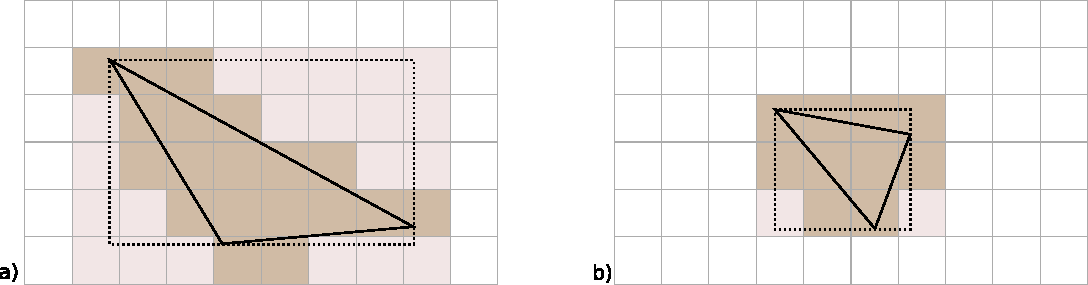
\includegraphics[width=1.0\textwidth]{images/gridconstr.pdf}
\caption[Fehler bei der Objektklassifizierung für regelmäßiges Gitter durch die AABBs]{Fehler bei der Objektklassifizierung für regelmäßiges Gitter durch die AABBs a) Einordnung lediglich aufgrund der AABB für bei, relativ großen Objekten zu mehr falschen Zuordnungen als bei b) relativ kleinen Objekten }
\label{fig:gridconstr}\end{center}
\end{figure}

\subsubsection{Effiziente Traversierung}
\label{sec:fastgrid}
Für die Traversierung sucht man nun die Voxel, die vom Strahl geschnitten werden. Danach werden lediglich diejenigen Objekte der Szene mit dem Strahl auf Schnitt getestet, die in den gefundenen Voxeln referenziert werden.

\begin{figure}\centering
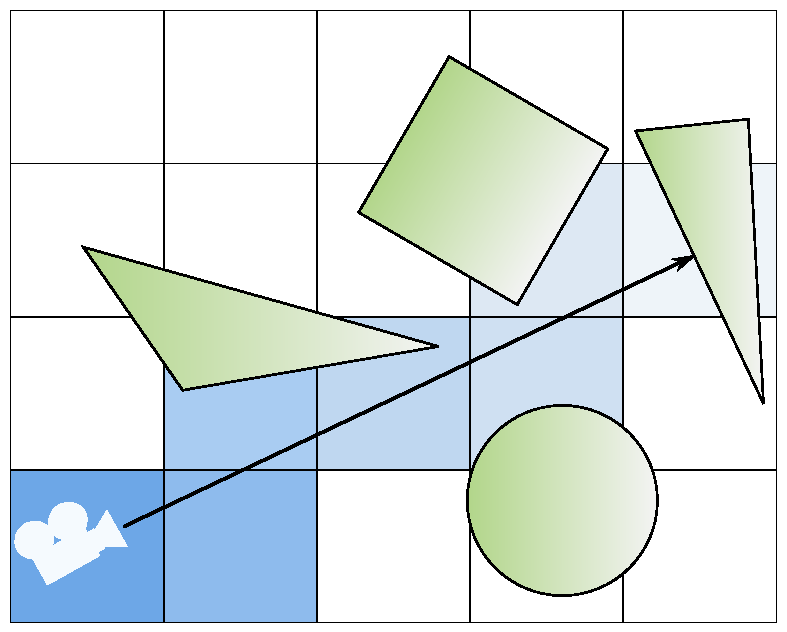
\includegraphics[width=0.5\textwidth]{images/gridtraversal.pdf}
\caption[Effiziente Gittertraversierung]{Effiziente Gittertraversierung}
\label{fig:gridtraversal}
\end{figure}

Durch die disjunkte und gleichmäßige Anordnung müssen unter Umständen nicht die Objekte \textit{aller} gefundenen Voxel gegen den Strahl getestet werden. Ein Objekt B das vom Strahlursprung aus gesehen hinter einem Objekt A liegt kann nicht einen näheren Schnittpunkt mit dem Strahl besitzen als Objekt A. Deswegen wird ein Algorithmus verwendet, der dem Bresenham-Algorithmus zum Zeichnen von Linien im 2D-Raum sehr ähnlich ist. Dieser von \cite{amanatides87} beschriebene Ansatz geht dabei wie folgt vor (siehe auch Abbildung \ref{fig:gridtraversal}:
\begin{enumerate}
 \item Bestimme den Voxel in dem der Ursprung des aktuellen Strahlabschnitts liegt (oder durch den der Strahl in das Gitter eintritt, wenn der Strahlursprung außerhalb des Gitters liegt)
 \item Teste den Strahl mit allen, in dem gefundenen Voxel referenzierten Objekten auf Schnitt 
 \item Wurde hier ein Schnitt gefunden, kann das Verfahren terminiert werden, da potentielle weitere Schnitte entlang des Strahls nur hinter dem gefundenen liegen können.
 \item Bestimme denjenigen Nachbarvoxel in den der Strahl als nächstes eintritt, und nimm den Eintrittspunkt als neuen Ursprung für den Strahl an.
 \item fahre mit 2. für den Nachbarvoxel fort
\end{enumerate}

Für Strahlsegmente, die außerhalb der AABB der Szene ihren Ursprung haben, muss zunächst der Eintrittspunkt des Strahls in das Gitter berechnet werden. Da vorher jedoch bereits der in Abschnitt \ref{sec:introstructs} erwähnte Test durchgeführt wurde, um festzustellen ob der Strahl die AABB der Szene überhaupt schneidet, kann der Eintrittspunkt durch Einsetzen von $t_{min}$ als $t$ in Gleichung \ref{eq:raysegment} leicht gefunden werden.

Der Voxel, in welchem sich ein Punkt im Gitter befindet, lässt sich durch ganzzahlige Division der Komponenten durch die jeweilige Breite eines Voxels bestimmen. Um herauszufinden, in welchen Voxel der Strahl als nächstes eintritt, muss zunächst bestimmt werden, ob sich der Strahl in jeder der drei Dimensionen in positiver oder in negativer Richtung ausbreitet. Da sich die Richtung eines Strahls während der Ausbreitung nicht ändert, genügt es einmal zu Beginn der Traversierung jeden Strahls die Vorzeichen der entsprechenden Komponente des Richtungsvektors zu betrachten.
Aus den Ausbreitungsrichtungen ergeben sich genau drei Voxel, in die der Strahl als nächstes eintreten kann.
Das Wissen über den Index des aktuellen Voxels und den Ursprung des aktuellen Strahlabschnitts, erlaubt es die Entfernungen zu den nächsten drei Voxeln wie folgt zu berechnen: ${\Delta}x = x_{next} - x_{current}$ (aquivalent für y und z). Durch Division der Entfernungen durch die entsprechende Komponente des Richtungsvektors des Strahls, lässt sich das kleinste $t$ aller drei Achsen bestimmen, für das der Strahl in einen weiteren Voxel eintritt: $t_x = \frac{{\Delta}x}{{d_R}^x}$(siehe Abbildung \ref{fig:nextcell})
\srcref{acceleration}{RegularGrid}{getFirstIntersection}

\begin{figure}\centering
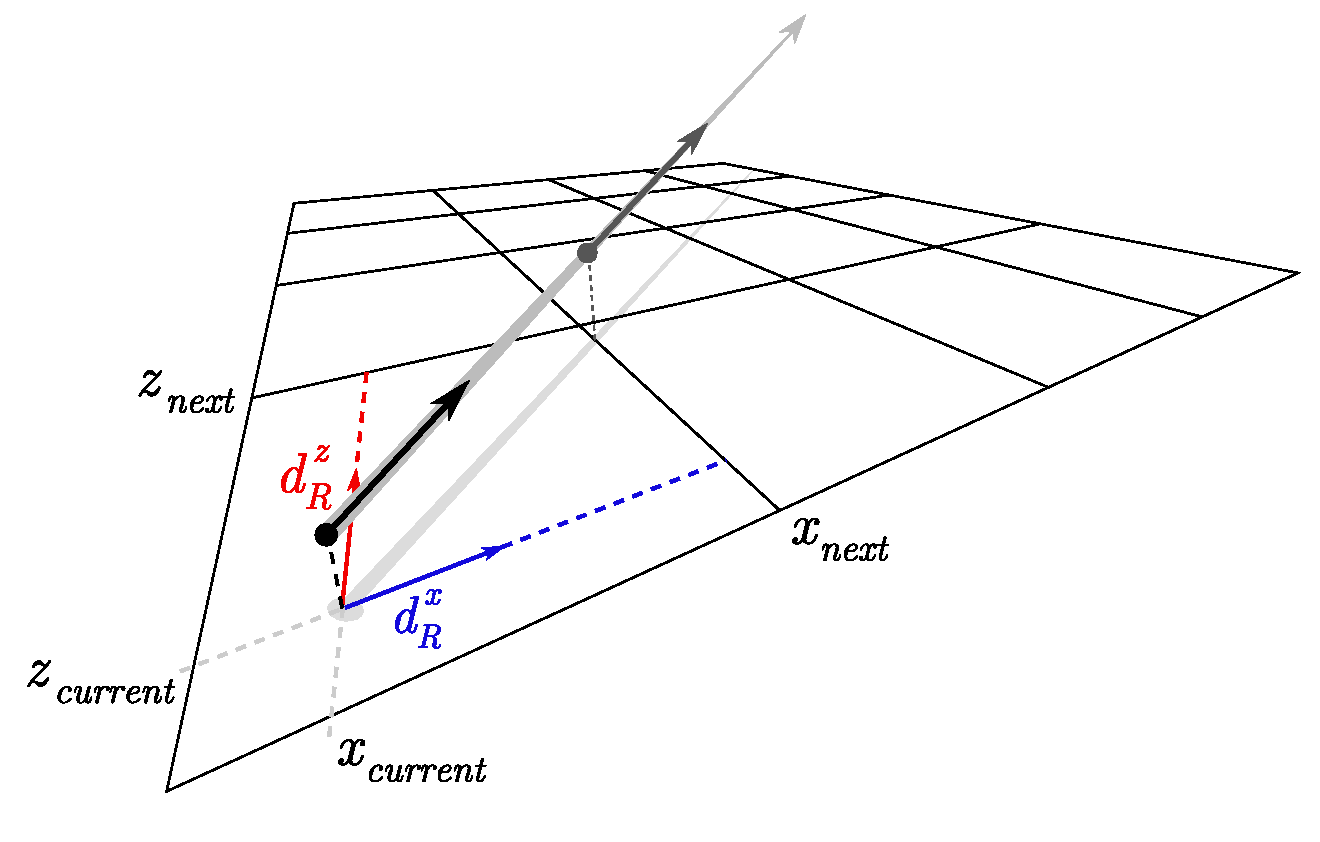
\includegraphics[width=0.6\textwidth]{images/nextcell.pdf}
\caption[Bestimmung des nächsten Voxels bei Gittertraversierung]{Bestimmung des nächsten Voxels in Strahlrichtung. Die Y-Achse wird hier vernachlässigt. Deswegen ergeben sich lediglich zwei potentielle nächste Voxel.}
\label{fig:nextcell}
\end{figure}


\subsubsection{Nachteile}

Durch die Verwendung von Gittern mit effizienter Traversierung können gegenüber dem naiven Ansatz zwar bereits viele unnötige Schnittests vermieden werden, dennoch zeigt das Verfahren in gewissen Konfigurationen signifikante Schwächen. Gerade in kargen Szenen muss der Algorithmus viele leere Zellen traversieren und dafür die oben beschriebenen Rechenschritte ausführen. Wird, um dem entgegenzuwirken, die Auflösung des Gitters verringert steigt die Wahrscheinlichkeit, dass Anhäufungen von kleinen Objekten komplett in einzelne Voxel fallen. Damit müssen Strahlen, welche durch diesen Voxel verlaufen, gegen sehr viele Objekte auf Schnitt getestet werden, was ja gerade verhindert werden soll.
Leider enthalten realistische Szenen oft viel leeren Raum, da die reale Welt vom Menschen meist so eingerichtet, dass er sich frei und bequem bewegen kann - was entsprechende freie Räume erfordert.
Die genannten Phänomene werden auch das \textit{Teapot-in-Stadium}-Problem genannt(Abbildung \ref{fig:stadium}).

\begin{figure}
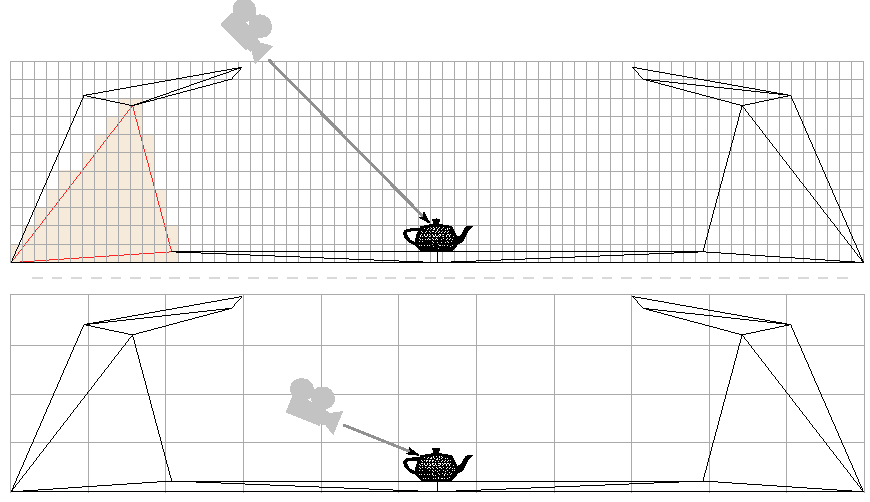
\includegraphics[width=1.0\textwidth]{images/stadium.pdf}
\caption[Teapot-in-Stadium bei regelmäßigen Gittern]{oben: Die feine Auflösung führt dazu, dass sehr viele leere Voxel traversiert werden müssen. Außerdem werden große Objekte von sehr vielen Voxeln referenziert, was zu enormen Speicherplatzbedarf führt. unten: Eine niedrige Auflösung führt dazu, dass viele Objekte in einzelnen Zellen liegen.}
\label{fig:stadium}
\end{figure}

\subsection{Octrees und hierarchische Gitter}

Das Problem bei dem zuvor beschriebenen Ansatz ist, dass leerer Raum genauso \textit{fein} aufgeteilt werden muss, wie Raumbereiche in denen sich viele kleine Objekte befinden. Um dem entgegenzuwirken kann der Raum zunächst in ein grobes Gitter aufgeteilt werden. Die Objekte der Szene werden, wie zuvor beschrieben, den zugehörigen Voxeln zugeordnet. An leeren Voxeln wird der Raum nicht weiter unterteilt. In Voxeln denen Objekte zugeordnet wurden, werden erneut, feinere Gitter eingefügt. Der Zuordnungsvorgang wird für die Objekte in diesem Voxel und die neu entstandenen Voxel des Subgrids wiederholt.
Dennoch muss die Frage nach der Wahl der Auflösung auch hier beantwortet werden. Dazu wurden in verschiedenen Arbeiten entsprechende Heuristiken entwickelt. Die Qualität dieser Verfahren hängt jedoch oft von der Szene und/oder von manuell zu wählenden Parametern ab, die mit guten \textit{Erfahrungswerten} belegt werden müssen.

Eine automatische Partitionierung der Szene wird durch die Verwendung von Octrees erreicht. Diese werden in \cite{Glassner88} erstmals für die Verwendung mit Raytracing vorgeschlagen. Im Prinzip sind die Octrees eine Untermenge der rekursiven Gitter. Jedes Gitter teilt den Raum in jeder Dimension in zwei Teile. Das heißt die AABB der Szene wird in ein Gitter aus acht Würfeln geteilt. Dann wird wie bei den rekursiven Gittern fortgefahren, indem jede nicht leere Gitterzelle in weitere acht Kuben unterteilt wird.

Die Traversierung verläuft ähnlich wie bei den nicht-hierarchischen Gittern. Jedoch müssen im Gegensatz zu den nicht-hierarchischen Gittern zunächst alle relevanten Voxel der Kindgitter getestet werden, bevor zu einem Nachbarvoxel fortgeschritten werden darf. Ein Vorteil der gleichmäßigen Unterteilung der Octrees ist, dass in einem beliebigen Traversionsschritt aus der Rekursionsstufe direkt auf die Größe eines Voxels geschlossen werden kann.

\subsection{BSP- \& Kd-Trees}

Eine weitere Verfeinerung der Raumaufteilung kann durch die Verwendung von binären Bäumen erreicht werden. Der Raum wird durch jeden der inneren Knoten des Baumes in lediglich zwei Voxel geteilt. Diese müssen, im Gegensatz zu Gittern, nicht die selbe Größe besitzen. \abbrev{BSP}{Binary Space Partitioning}Binary Space Partitioning(BSP)-Trees werden das erste Mal für die Computergrafik in \cite{Fuchs80} verwendet. Die dort ausschließlich für Polygone entwickelte Version lässt sich aber einfach für beliebige Primitive erweitern. Durch die Tatsache, dass die Trennebene beliebig gewählt werden kann, sind die BSP-Trees in der Lage sich besser an die Geometrie anzupassen als gleichmäßige Verfahren.

Für das Raytracing hat sich ein Spezialfall der BSP-Trees als besonders effizient herausgestellt: die so genannten Kd-Trees (auch axis-aligned oder rectilinear BSP-Trees). Sie grenzen sich von den allgemeinen BSP-Trees durch die Bedingung ab, dass die trennende Ebene in einem inneren Knoten immer orthogonal zu einer der drei Hauptachsen sein muss. Neben einfacherer Konstruktion und Traversierung lässt sich der Baum auch kompakter als ein beliebiger BSP-Tree speichern. Für einen inneren Knoten müssen, neben den Referenzen auf die Kindknoten, lediglich die Achse ${x,y,z}$ und ein Skalar - die Position der Ebene auf der Achse - gespeichert werden müssen. Die Blätter des Baumes referenzieren jeweils die Liste der Objekte die den Voxel überlappen, der sich aus der Raumteilung der Vorgängerknoten ergibt. Ein Kd-Tree lässt sich wie in Quelltext \ref{kddef} definieren.

\begin{lstlisting}[float,caption=Beschreibung der Kd-Tree Daten\-struk\-tur in erweiterter Backus-""Naur-""Form,label=kddef]
 KdTree    = InnerNode | Leaf
 InnerNode = Axis Position KdTree KdTree
 Axis      = 'x' | 'y' | 'z'
 Position  = float
 Leaf      = { Primitiv }\end{lstlisting}

\subsubsection{Traversierung}
\begin{figure}\centering
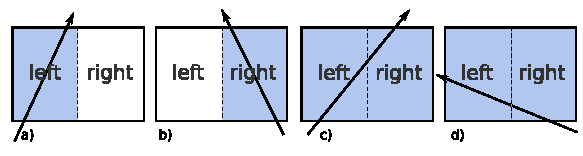
\includegraphics[width=1.0\textwidth]{images/kdtrav.pdf} 
\caption[Fallunterscheidung bei Traversierung eines BSP-Trees]{a) nur der linke Kindknoten wird geschnitten und muss besucht werden, b) nur der rechte Kindknoten wird geschnitten, c) beide Knoten müssen besucht werden, der linke wird zuerst geschnitten und muss daher zuerst besucht werden, d) beide Knoten werden geschnitten, der rechte Knoten muss als erstes besucht werden.}
\label{fig:kdtrav}
\end{figure}

Ein Grund warum binäre Bäume sich so großer Beliebtheit erfreuen ist, dass die Traversierung einfacher ist als bei mehrstelligen Bäumen oder hierarchischen Gittern, was eine effiziente Implementierung begünstigt. Im Gegensatz zu Octrees, wo bis zu vier der acht Kindvoxel (in verschiedenen Reihenfolgen) von einem Strahl geschnitten werden können, tritt beim Kd-Tree lediglich einer von vier möglichen Fällen pro Knoten auf (siehe Abbildung \ref{fig:kdtrav}):
\begin{enumerate}
 \item Es wird nur der vordere Voxel geschnitten
 \item Es wird nur der hintere Voxel geschnitten
 \item Es wird zuerst der hintere und dann der vordere Voxel geschnitten
 \item Es wird zuerst der vordere und dann der hintere Voxel geschnitten
\end{enumerate}

Zur Beantwortung der Strahlanfragen müssen die Knoten des Baums, von der Wurzel an beginnend, rekursiv besucht werden. Erreicht der Algorithmus ein Blatt, wird der Strahl mit allen im Blatt enthaltenen Objekten auf Schnitt getestet.
Für einen inneren Knoten werden lediglich die Kindknoten besucht, deren Voxel vom Strahl geschnitten wird. Für den Fall, dass beide Knoten vom Strahl geschnitten werden, ergibt sich die Traversierungsreihenfolge der Kindknoten aus der Reihenfolge in der der Strahl die Voxel der Kindknoten schneidet.
Bei Beachtung der Traversierungsreihenfolge kann der Algorithmus bereits nach dem Besuch des ersten Knotens terminiert werden, wenn ein Schnittpunkt mit einem Objekt aus diesem Teilbaum gefunden wurde. Durch die disjunkte räumliche Anordnung der Voxel ist garantiert, dass jeder weitere potentielle Schnitt, der im Voxel des \textit{anderen} Kindknotens liegt, hinter dem bereits gefundenen liegen muss.

Für die Bestimmung der Traversierungsreihenfolge genügt es das Vorzeichen einer Komponente des Richtungsvektors zu betrachten. Die interessante Komponente ist die, entlang welcher der Voxel des aktuellen Knotens geteilt wird. Der Teilbaum, der als erstes traversiert werden muss, wird dabei als \textit{nah} und der zweite als \textit{ferner} Teilbaum bezeichnet.
Ob der nahe Teilbaum überhaupt besucht werden muss, lässt sich über die relative Position des Strahlursprungs zur Trennebene bestimmen: Liegt er in Ausbreitungsrichtung hinter der Trennebene, kann der nahe Teilbaum übersprungen werden. Der ferne Teilbaum muss nur dann nicht traversiert werden, wenn der Strahl diesen außerhalb des Strahlsegments schneidet. Dafür wird die parametrische Distanz des Ursprungs zur Trennebene mit dem Parameter $t_{max}$ des Strahlsegments verglichen. 
Quellcode \ref{kdtravcode} zeigt das beschriebenen Vorgehen bei der Traversierung in Pseudocode.
\srcref{accelleration}{KdTreeSimple}{getFirstIntersection}

\begin{lstlisting}[float,caption=Traversierung eines Kd-Trees,label=kdtravcode]
Intersection getIntersection(KdTree node, Ray ray){
 if ( node.isLeaf() ) {
   return node.primitives.intersect(ray);
 } else {
  KdTree near, far;
  if ( r.direction[node.axis] > 0.0 )
    near = left ; far = right;
  else
    near = right; far = left;
  }
  d = (node.splitPos - ray.origin.[node.axis]) / ray.direction[node.axis];
  Intersection result; // wird leer initialisiert
  if ( d > 0 ) // der 'nahe' Knoten muss besucht werden
    result = getIntersection(near, ray);
  if ( ! result.isEmpty() ) // ggf. fruehe Terminierung
    return result;
  if ( d < ray.tmax ) // nur falls 'ferner' Voxel geschnitten wird
    return getIntersection( far, ray);
  return result;
 }
}\end{lstlisting}

\begin{figure}\centering
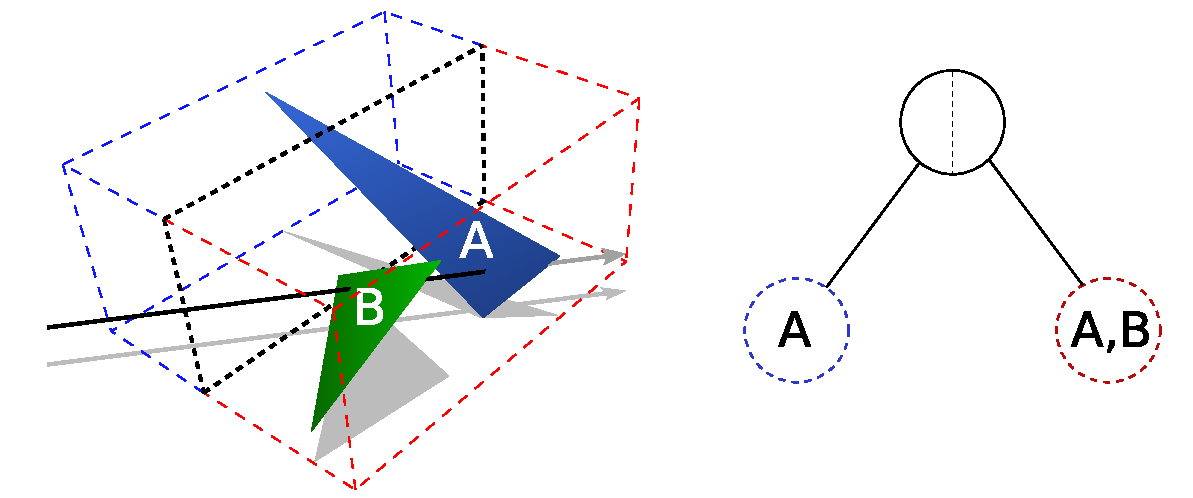
\includegraphics[width=0.9\textwidth]{images/mailboxing.pdf} 
\caption[Keine Terminierung bei Schnitt außerhalb des aktuellen Voxels]{links: Der blaue Voxel wird als erstes getestet, da er als erstes vom Strahl geschnitten wird. Es wird zwar ein Schnittpunkt mit Dreieck A gefunden, das Verfahren darf aber nicht terminiert werden, da der Schnittpunkt nicht innerhalb des blauen Voxels liegt - denn der rote Voxel enthält noch einen Schnittpunkt mit B der näher am Ursprung liegt. rechts: Der Baum zu der Geometrie besteht aus der Wurzel die die gesamte AABB in den blauen Voxel(der lediglich A enthält) und den roten Voxel(der A und B) enthält, teilt.}
\label{fig:mailbox}
\end{figure}

Die frühe Terminierung der Traversierung darf allerdings nur dann vorgenommen werden, wenn der gefundenen Schnittpunkt innerhalb des Voxels des aktuell traversierten Teilbaums liegt. Befindet sich der Schnittpunkt außerhalb des aktuellen Voxels, können anderenfalls potentielle, nähere Schnittpunkte nicht gefunden werden (siehe Abbildung \ref{fig:mailbox}). Kritisch sind dabei die Fälle, in denen der bei der Traversierung des \texttt{vorderen} Teilbaumes gefundene Schnitt, tatsächlich im Voxel des \textit{hinteren} Teilbaums liegt. Dieses lässt sich leicht feststellen, indem man den Abstand des Schnittpunktes zum Strahlursprung mit dem Abstand zur Trennungsebene vergleicht.

Wie bereits in Abschnitt \ref{sec:dsijointstructs} angedeutet führt das dazu, dass ein Objekt mehrmals mit dem gleichen Strahl auf Schnitt getestet werden kann, was gerade bei komplexen Objekten vermieden werden sollte. Beim Mailboxing, wie in \cite{Benthin06} beschrieben, wird jedem Strahl eine eindeutige Identifikationsnummer(ID) zugewiesen. Bei dem Schnitttest mit einem Objekt, speichert das Objekt die Strahl-ID. So kann bei einem wiederholten Test festgestellt werden, dass der Schnittpunkt bereits berechnet wurde, und muss so nicht wiederholt werden.

\subsubsection{Konstruktion}

Bei der top-down Konstruktion eines kd-Trees wird die AABB der Szene durch eine achsenparallele Trennebene in zwei Subvoxel unterteilt. Die Objekte werden dann dem linken, rechten oder beiden Subvoxeln zugeordnet, je nachdem welchen der Subvoxel ein Objekt überlappt. Ein Abbruchkriterium ist eine minimale Anzahl an Objekten für die ein Voxel nicht weiter unterteilt werden soll. Um den Speicherbedarf zu begrenzen wird meistens zusätzlich eine maximale Rekursionstiefe als Abbruchbedingung festgelegt.
Quelltext \ref{buildkd} zeigt einen rekursiven Algorithmus zur Konstruktion eines Kd-Trees.\srcref{accelleration}{KdTreeSimple}{construct}


\begin{lstlisting}[mathescape,float,caption=Eine einfache Version eines Konstruktionsalgorithmus für kd-Trees,label=buildkd]
KdTree buildKdTree( List<Primitive> primitives, AABB voxel ) {
  if ( terminationCriterionMet() ) {
    return Leaf( primitives );
  } else {
    ( splitPosition, splitAxis ) = heuristic.getSplit( primitives, voxel );
    ( $V_{left}, V_{right}$ ) = voxel.split( splitPosition, splitAxis );
    List<Primitive> $P_{left}, P_{right}$;
    foreach ( primitive in primitives ) {
      if ( primitive.overlaps( $V_{left}$) )
        $P_{left}$.add( object );
      if ( primitive.overlaps( $V_{right}$) )
        $P_{right}$.add( object );
    }
    return InnerNode ( splitAxis, splitPosition,
                          buildKdTree(left, $V_{left}$),
                          buildKdTree(right, $V_{right}$) )
  }
}\end{lstlisting}

Die Wahl der Achse und Position der Schnittebene wird an eine \textit{Heuristik} delegiert. Eine der einfachsten Heuristiken für diesen Zweck wählt immer den Mittelpunkt der längsten Achse der AABB. Das führt zu einer ähnlichen Raumaufteilung wie bei den Octrees. Diese Raumaufteilung nutzt nicht die Fähigkeit der BSP-Trees sich an die Szenengeometrie anzupassen und unterliegt deswegen Heuristiken, die dies ausnutzen. Diese Beobachtung wird durch die statistische Untersuchungen in \cite{Havran00} bestätigt.

Um die Objekte bei der Konstruktion in den jeweils linken oder rechten Teilbaum einzusortieren, muss bestimmt werden welche Voxel der Kindknoten von dem Objekt geschnitten werden.
Man kann sich hierbei auf eine Betrachtung der AABBs der Objekte beschränken, um einen aufwändigen Objekt-AABB-Schnitttest zu vermeiden.
Dies führt aber, wie bereits bei den Gittern in \ref{sec:gridconstruction}, dazu, dass Objekte auch in Voxel einsortiert werden, die zwar die AABB des Objekts, aber nicht vom Objekt selbst geschnitten werden. Neben dem erhöhten Speicherplatzbedarf führt dies auch zu unnötigen Strahl-Objekt-Schnittests in der Traversierungsphase.

Für Dreiecke und AABBs gibt es zahlreiche Schnittestalgorithmen. Für die Tests die zur Klassifizierung bei der Konstruktion eines Kd-Trees benötigt werden ist es jedoch möglich einen weniger allgemeinen, aber dafür effizienteren Algorithmus anzuwenden wie er von \cite{Waechter08} beschrieben wird. 
Dabei werden folgende Annahmen ausgenutzt:
\begin{itemize}
 \item Ein Dreieck überlappt immer den aktuellen Voxel (zumindest teilweise)
 \item Ein Dreieck, welches den aktuellen Voxel überlappt muss auch mindestens einen der beiden Subvoxel überlappen.
 \item Wenn die AABB eines Dreiecks komplett auf einer Seite der Trennebene liegt, kann es nur den auf dieser Seite liegenden Voxel überlappen.
 \item Wenn das Dreieck genau in (parallel zu, und an der Stelle) der Trennebene liegt muss eine Heuristik entscheiden in welche der beiden Voxel das Dreieck einsortiert wird.
\end{itemize}

Der Algorithmus geht dann wie folgt vor. Es werden zunächst zwei Trivialfälle getestet
\begin{enumerate}
 \item Prüfe ob das Dreieck in der Trennebene liegt
 \item Prüfe ob die AABB des Dreiecks vollständig vor oder hinter der Trennebene liegt.
\end{enumerate}
Falls einer der beiden Fälle zutrifft, muss das Dreieck direkt in einen der Teilbäume einsortiert werden.
Andernfalls muss festgestellt werden, ob das Dreieck den Querschnitt des Voxels, an der Stelle der Trennebene ($A_{split}$), schneidet. Dazu werden die folgenden Schritte ausgeführt:
\begin{enumerate}
 \item Bestimme den Vertex des Dreiecks der sich \textit{alleine} auf einer Seite der Trennebene befindet.
 \item Über die Entfernung $d$ zur Trennebene (siehe Abbildung \ref{fig:splitvoxel}) lassen sich die beiden Schnittpunkte $S_1, S_2$ des Dreiecks mit der (unbegrenzten) Trennebene bestimmen.
 \item Falls das achsenparallele Viereck dessen Diagonale die Strecke $S_1-S_2$ darstellt, den Querschnitt des Voxels ($A_{split}$) nicht schneidet, kann das Dreieck sofort \textit{einem} der beiden Voxel zugeordnet werden.
 \item Andernfalls wird zunächst eine Senkrechte $\vec{n}$ zu $S_1-S_2$ bestimmt. Über die Komponenten von $n$ lässt sich die Ecke $p_1$ des Rechtecks $A_{split}$ bestimmen, welche am weitesten von $S_1-S_2$ entfernt ist. Falls die Gerade auf der $S_1-S_2$ liegt zwischen dieser und der gegenüberliegenden Ecke liegt \textbf{muss} $S_1-S_2$ das Rechteck schneiden und muss in beide Voxel einsortiert werden. Andernfalls wird das Dreieck wieder nur in einen Voxel einsortiert. Zur Bestimmung ob die beiden Ecken auf der selben Seite der Geraden liegen genügt es die Vorzeichen der folgenden Produkte: $(S_1 - p_1) * \vec{n}$ und $(S_1 - p_2) * \vec{n}$.
\end{enumerate}

\begin{figure}\centering
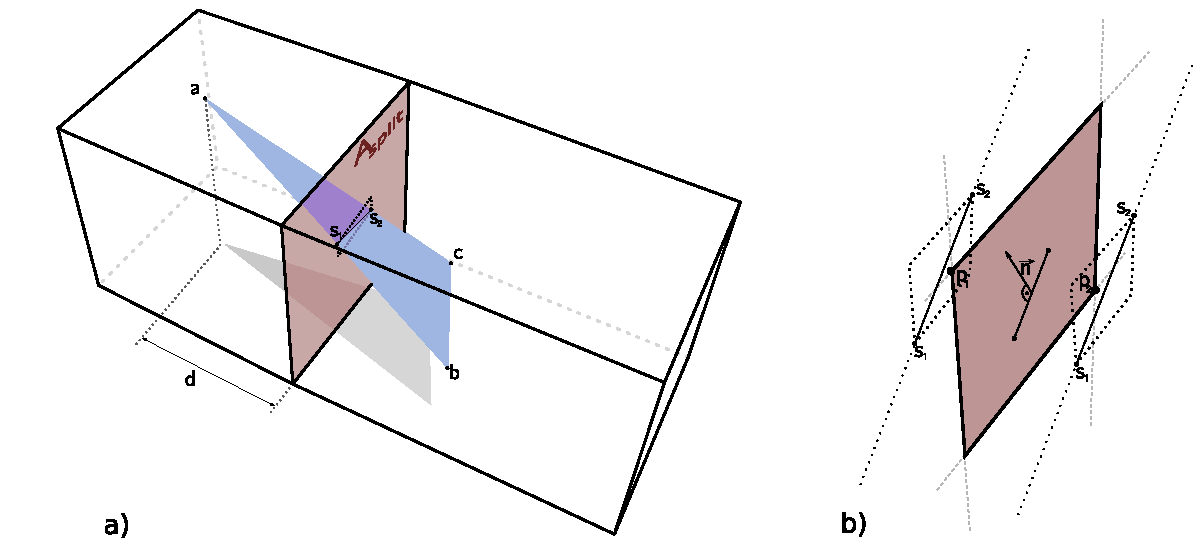
\includegraphics[width=1.0\textwidth]{images/split.pdf} 
\caption[Effizienter Dreieck/Subvoxel Schnittest]{a) Das Dreieck muss beiden Voxeln zugeordnet werden, da $A_{split}$ von $S_1-S_2$ geschnitten wird. b) Für die äußeren beiden Fälle schneidet die Gerade das Rechteck nicht, somit kann auch $S_1-S_2$ das Rechteck nicht schneiden.}
\label{fig:splitvoxel}
\end{figure}

\subsubsection{Surface Area Heuristic}

Die Effizienz der Strahlanfragen an einen Kd-Tree hängt maßgeblich von der Qualität der Raumaufteilung ab, die durch den Baum vorgenommen wird. Globale, regelmäßige Aufteilungen führen zu den bei Gittern erwähnten Problemen. Auch eine Wahl der Schnittebenen bei denen sich ein möglichst balancierter Binärbaum ergibt - also die Platzierung der Trennungsebene am Objektmedian - führt nicht zu einem idealen Baum für Strahlanfragen. Diese Konstruktion ist zwar für allgemeine Suchbäume effizient, geht aber davon aus, dass alle Knoten gleichhäufig besucht werden. Da für große Voxel die Wahrscheinlichkeit, dass sie von einem Strahl getroffen werden aber höher ist, ist diese Annahme so nicht gültig. Weiter wird im Gegensatz zu Suchen auf allgemeinen binären Suchbäumen auch nicht genau ein Pfad von der Wurzel zu dem gesuchten Blatt besucht. Vielmehr müssen unter Umständen an mehreren inneren Knoten beide Teilbäume interpretiert werden, wenn im ersten Teilbaum kein Schnittpunkte gefunden wurde.\citep{Wald04}

Die Heuristiken welche die beste Raumaufteilung liefern, berechnen die Güte einer potentiellen Trennungsebene mit Hilfe einer Kostenfunktion (\cite{Havran00}). Die bekannteste Heuristik, die eine solche Kostenfunktion zur Verfügung stellt, ist die \abbrev{SAH}{Surface Area Heuristic}Surface Area Heuristic(SAH). Ein guter Baum ermittelt den gesuchten Schnittpunkt beziehungsweise, dass es keinen Schnittpunkt gibt, für einen beliebigen Strahl mit möglichst wenig Traversierungsschritten und möglichst wenig Schnittests. Für die SAH wird angenommen, dass Strahlen sich gleichverteilt im Raum befinden und in ihrem Verlauf nicht durch Objekte unterbrochen werden. Aus dieser Vereinfachung lässt sich eine Beziehung zwischen der Oberfläche eines Voxels und der Wahrscheinlichkeit, dass dieser von einem Strahl getroffen wird, herstellen: Je größer die Oberfläche eines Voxles ist, desto wahrscheinlicher ist es, dass dieser von einem Strahl getroffen wird. Ein guter Baum enthält möglichst viele, möglichst große, leere Zellen - und diese möglichst nah an der Wurzel. 

Um die Kostenfunktion für die Positionierung der Trennebene eines Voxels aufstellen zu können trifft die SAH folgende Annahmen:
\begin{itemize}
 \item Strahlen sind gleichmäßig im Raum verteilt
 \item Strahlen sind Geraden(ohne Start- und Endpunkt) und werden nicht unterbrochen
 \item Die Kosten für den Schnitt mit einem Objekt $C_i$ und die Kosten für einen Traversierungsschritt $C_t$ sind bekannt
\end{itemize}

Durch diese Annahmen lässt sich aus der Oberfläche $A_{V_{sub}}$ eines Teilvoxels $V_sub \subset V$ auf die Wahrscheinlichkeit $P$ schließen, dass von ein Strahl der $V$ trifft auch $V_sub$ trifft\ref{eq:sah1}
\begin{equation}
P(V, V_{sub}) = \frac{A_{V_{sub}}}{A_V}
 \label{eq:sah1}
\end{equation}

Für die Kostenfunktion wird zunächst der Trivialfall betrachtet: Wie hoch sind die Kosten für einen Strahl der die AABB der Szene trifft wenn der Wurzelknoten eines Kd-Trees direkt ein Blatt ist, und demnach alle Primitive enthält? 
Dies entspricht der naiven Lösung aus \ref{sec:naiv}, denn jedes Objekt muss gegen den Strahl getestet werden.
Die Kosten sind demnach $C_leaf = N * C_i$, wobei $N$ der Anzahl der Objekte entspricht.

Nach Bestimmung der Position der Trennebene für einen Voxels werden die Objekte den entstehenden zwei Subvoxeln zugeordnet. Die Kosten die sich für die Schnitttests ergeben werden mit den jeweiligen Trefferwahrscheinlichkeiten der Subvoxel gewichtet. Das heißt eine Trennung, bei der ein Voxel mit sehr wenigen Objekten, mit einer hohen Wahrscheinlichkeit getroffen wird, ergibt einen sehr \textit{günstigen} Knoten. Zusätzlich kommen dann die Kosten für den Traversierungsschritt hinzu, die im Verhältnis zu einem Objekt-Strahlschnittest aber sehr niedrig sind. Die Kosten $C$ für die Trennung eines Voxels $V$ durch die Ebene $q$ lassen sich dann wie folgt in Gleichung \ref{eq:nodecost} bestimmen:

\begin{equation}
C_V(q) = C_t + P(V, V_{left}) * C_{left} * C_i + P(V, V_{right}) * C_{right} * C_i
 \label{eq:nodecost}
\end{equation}

Für eine gute Raumaufteilung muss ein möglichst günstiger Baum gefunden werden. Um die Kosten für einen kompletten Baum zu berechnen müssen die Positionen aller Trennebenen bekannt sein. Denn nur so lässt sich $P$, und damit die Kosten, für die tiefer liegenden Voxel bestimmen. Dies steht jedoch im Widerspruch dazu, dass die Kostenfunktion bereits in den oberen Ebenen des Baumes genutzt werden soll um eben die beste Position für die Trennebenen zu finden.

Um dennoch eine Abschätzung vornehmen zu können, nimmt man für eine potentielle Trennebene an, dass die entstehenden Subvoxel nicht weiter unterteilt werden. Diese, sehr grobe, Abschätzung überschätzt die tatsächlich für die Subvoxel entstehenden Kosten, da diese mit hoher Wahrscheinlichkeit weiter unterteilt werden - und damit günstiger werden. Die Vorgehensweise hat sich in der Praxis aber dennoch als wirksames Indiz für gute Trennebenen erwiesen.

Beim Vergleich zweier potentieller Trennebenen muss mehrmals Gleichung \ref{eq:sah1} für die Kostenbestimmung ausgewertet werden. Da alle potentiellen Ebenen eines Knotens den gleichen Voxel teilen, und lediglich das relative Verhältnis der Kosten zueinander interessant ist, kann auf die Division durch $A_V$ verzichtet werden. Eine weitere Vereinfachung der Berechnung der Kosten lässt sich erreichen wenn es nur einen Typ von Objekten (zum Beispiel Dreiecke) gibt. In diesem Fall kann $C_i$ durch $1$ ersetzt werden. So ergibt sich zur Berechnung der relativen Kosten in einem Knoten Gleichung \ref{eq:relsah}.

\begin{equation}
{C_V}_{rel}(q) = C_t + V_{left} * N_{left} + V_{right} * N_{right}
 \label{eq:relsah}
\end{equation}

Für plane Objekte kann zusätzlich der Sonderfall eintreten, dass sie \textit{in} der Trennebene liegen. Sie müssen aber trotzdem einen der beiden Teilbäume zugeordnet werden. Eine Zuordnung in beide Teilbäume ist zwar nicht falsch, führt aber zu weniger effzienten Strahlanfragen.
\citep{WaldHavran06} empfehlen diesen Fall extra zu verfolgen und anschließend zu untersuchen ob einer der Teilbäume keine Objekte enthält. Plane Objekte die in der Trennebene liegen werden dann dem nicht-leeren Teilbaum zugeordnet.

\subsubsection{Zusätzliches Terminierungskriterium}

Neben der Positionierung der Trennebene lässt sich die SAH zusätzlich zur Einführung einer besseren Abbruchbedingung für die rekursive Konstruktion einsetzen. Durch Gleichung \ref{eq:nodecost} lassen sich die Kosten für den Fall berechnen, dass der aktuelle Voxel nicht weiter unterteilt wird. Sind die Kosten, die durch die Trennung mit der günstigsten Trennebene entstehen, höher als den Knoten nicht zu teilen, lohnt es sich nicht die Unterteilung fortzusetzen.
Da die lokale Bestimmung dazu tendiert die Kosten für die entstehenden Subvoxel zu überschätzen kann es erforderlich sein bei dem Vergleich einen entsprechenden Faktor einzubeziehen um ein vorzeitiges Terminieren zu verhindern.


\subsubsection{Kanditatengenerierung für Trennebenen}

Da es auf einer Achse unendlich viele mögliche Positionen für eine Trennebene gibt, muss für die Kandidaten eine sinnvolle Untermenge gewählt werden. Für diese kann dann die Kostenfunktion der SAH ausgewertet und der günstigste Kandidat verwendet werden. Bei Betrachtung der Komponenten der Kostenfunktion (siehe Abbildung \ref{fig:sahdiagr}) stellt sich heraus, dass das gesuchte Minimum nur an bestimmten Stellen liegen kann. Diese befinden sich jeweils an den Minima beziehungsweise Maxima der AABBs der Objekte (für Objekte die teilweise außerhalb des Voxels liegen trifft dies auch für die Schnittpunkte der Objektkanten mit dem Voxel zu: siehe Abbildung \ref{fig:splitmiss}). Zwischen zwei benachbarten Stellen kann kein Minimum der Kostenfunktion liegen \citep{WaldHavran06}.

\begin{figure}
\begin{center}
\begin{asy}
import graph;

picture pic;
real xsize=190, ysize=180;
size(pic,xsize,ysize,IgnoreAspect);


  real[] xd0={0.0, 2.2, 3.4};
  real[] yd0={2.1, 0.9, 2.9};

  real[] xd1={3.8, 5.0, 5.7};
  real[] yd1={2.7, 3.1, 2.5};

  real[] xd2={4.6, 5.8, 6.8};
  real[] yd2={1.7, 0.1, 2.3};

   real[] x={0.0, 3.4, 3.8, 4.6, 5.7, 6.8};
   real[] x2=       {0.0, 3.4, 3.4, 3.8, 3.8, 4.6, 4.6, 5.7, 5.7, 6.8};
   real[] primleft= {1.0, 1.0, 1.0, 1.0, 2.0, 2.0, 3.0, 3.0, 3.0, 3.0};
   real[] primright={3.0, 3.0, 2.0, 2.0, 2.0, 2.0, 2.0, 2.0, 1.0, 1.0};
   real[] aleft=2*x2 + 8.8;
   real[] aright=2*(6.8 - x2) + 8.8;
   real[] cost=(aleft/22.4)*primleft*4.0 + (aright/22.4)*primright*4.0;

   draw(pic,graph(new real[]{xd0[0], xd0[1]},new real[]{yd0[0], yd0[1]}), gray(0.9));
   draw(pic,graph(new real[]{xd0[0], xd0[2]},new real[]{yd0[0], yd0[2]}), gray(0.9));
   draw(pic,graph(new real[]{xd0[1], xd0[2]},new real[]{yd0[1], yd0[2]}), gray(0.9));

   draw(pic,graph(new real[]{xd1[0], xd1[1]},new real[]{yd1[0], yd1[1]}), gray(0.9));
   draw(pic,graph(new real[]{xd1[0], xd1[2]},new real[]{yd1[0], yd1[2]}), gray(0.9));
   draw(pic,graph(new real[]{xd1[1], xd1[2]},new real[]{yd1[1], yd1[2]}), gray(0.9));

   draw(pic,graph(new real[]{xd2[0], xd2[1]},new real[]{yd2[0], yd2[1]}), gray(0.9));
   draw(pic,graph(new real[]{xd2[0], xd2[2]},new real[]{yd2[0], yd2[2]}), gray(0.9));
   draw(pic,graph(new real[]{xd2[1], xd2[2]},new real[]{yd2[1], yd2[2]}), gray(0.9));

   draw(pic, "\footnotesize$N_{left}$", graph(x2,primleft), blue, "$N_{left}$");
   draw(pic, "\footnotesize$N_{right}$",graph(x2,primright),red);
xaxis(pic,"\footnotesize Position der Trennebene $p$",Bottom,LeftTicks(Label(fontsize(8)),x),EndArrow);
yaxis(pic,"N",Left,
      RightTicks(Label(fontsize(8)),new real[]{0,1,2,3}),EndArrow);

//attach(pic,legend(pic)); 

picture pic2;
size(pic2,xsize,ysize,IgnoreAspect);
   draw(pic2, "\footnotesize$A_{V_{left}}$",graph(x2,aleft),red);
   draw(pic2, "\footnotesize$A_{V_{right}}$",graph(x2,aright),blue);
   draw(pic2, "\footnotesize$C_{V}(p)$",graph(x2,cost),green);
xaxis(pic2,"\footnotesize Position der Trennebene $p$",Bottom,LeftTicks(Label(fontsize(8)),x),EndArrow);

yaxis(pic2, "", Left, 0, 25, currentpen, RightTicks(Label(fontsize(8)), new real[]{5,10,15,20}), EndArrow, Below);
add(pic.fit(),(0,0),W);
add(pic2.fit(),(5mm,0),E);
\end{asy}
\caption[Begrenzte Anzahl von sinnvollen Positionen für Trennebene]{links: Anzahl der Objekte im rechten bzw. linken Subvoxel bei entsprechender Positionierung der Schnittebene. rechts: Die Oberflächen (bzw. hier Umfänge, da 2D) der Subvoxel bei entspr. Trennung. In grün die lokale Kostenfunktion}\label{fig:sahdiagr}
\end{center}
\end{figure}

\begin{figure}\centering
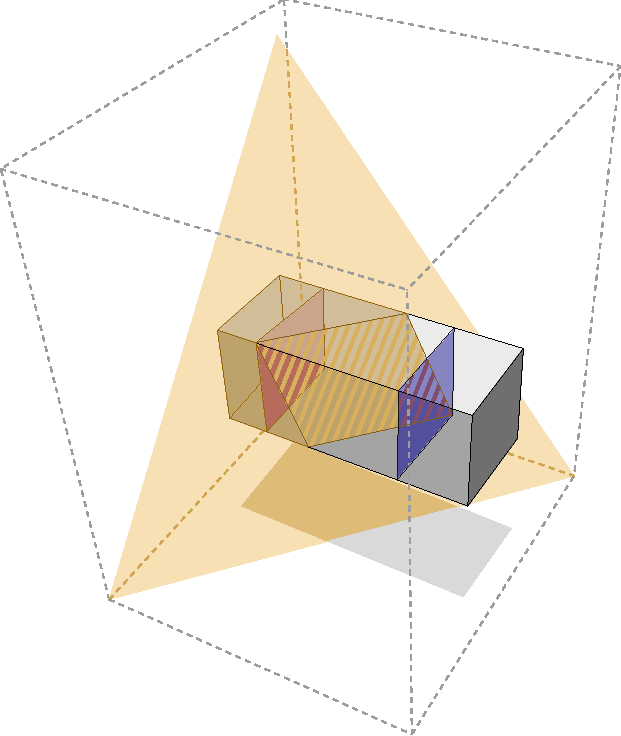
\includegraphics[width=0.4\textwidth]{images/splitmiss.pdf} 
\caption[Fehlende Kandidaten bei ausschließlicher Betrachtung der AABBs]{Die Minima/Maxima der Objekte als Trennkandidaten zu verwenden reicht nicht aus. Die rote und blaue Position für Schnittebenen sind wichtige Kandidaten die an den Minima/Maxima der Schnittkanten des Objektes mit dem Voxel zu finden sind. Da der Voxel komplett in der AABB des Dreiecks liegt würde in diesem Fall sonst gar kein Kandidat gefunden.}
\label{fig:splitmiss}
\end{figure}

Um die beste Position für die Trennebene zu finden, müssen also zunächst die Grenzen der AABBs der Objekte entlang jeder Achse gesammelt werden. Danach muss für jede der gefundenen Stellen die Kostenfunktion der SAH ausgewertet werden. Dabei wird verfolgt welche Position die bisher niedrigsten Kosten verursacht hat (siehe auch Quelltext \ref{perfectsplits}).\srcref{acceleration}{KdTreeSAHNaive}{construct}

\begin{lstlisting}[float,mathescape=true,caption=Suche nach der besten Trennebene in $O(n^2)$  ,label=perfectsplits]
(float, Axis) searchBestSplitPos(AABB voxel, List<Primitive> primitives) {
  List<float> splitCandidates[{x,y,z}];
  foreach (primitive in primitives) {
    AABB clippedBox = primitive.clipTo(voxel);
    foreach ( axis in {x,y,z} ) {
      splitCandidates[axis].add(clippedBox.min[axis]);
      splitCandidates[axis].add(clippedBox.max[axis]);
    }
  }

  float bestCost = $\infty$;
  float bestPos;
  Axis bestAxis;
  foreach ( axis in {x,y,z} ) {
    foreach ( candidatePosition in splitCandidates ) {
      List<Primitive> $N_{left}, N_{right}$
      foreach ( primitive in primitives ) {
        if ( pimitive.AABB.min[axis] < candidatePosition )
          ++$N_{left}$
        if ( pimitive.AABB.max[axis] >= candidatePosition )
          ++$N_{right}$;
      }
      ( $V_{left}$, $V_{right}$ ) = voxel.split( axis, candidatePosition );
      float currentCost = $C_t + V_{left}$.surface() $* N_{left} + V_{right}$.surface()$ * N_{right}$;
      if ( currentCost < bestCost ) {
        bestCost = currentCost;
        bestPos = candidate;
        bestAxis = axis;
      }
    }
  }
  return (bestPos, bestAxis);
}

\end{lstlisting}

\section{Partitionierung der Objektmenge}
Grundlegend anders als die disjunkten Raumaufteilungsverfahren wird bei der Anwendung von Bounding Volume Hierarchies(BVH)\abbrev{BVH}{Bounding Volume Hierarchies} vorgegangen. Hier wird anstatt die AABB der Szene, die Menge der Objekte partitioniert. 

Bei der top-down Konstruktion wird die Menge der Objekte in zwei (für binäre Bäume, sonst auch mehr) disjunkte Teilmengen zerlegt. Für jede Teilmenge wird ein neuer Knoten erstellt. Dieser Vorgang wird für jeden neuen Knoten wiederholt bis nur noch ein Objekt in den entstehenden Teilmengen vorhanden ist. Für dieses wird dann ein Blattknoten angelegt. Nach der Erzeugung der Blätter wird für jeden Knoten die gemeinsame AABB der Kindknoten berechnet. Die AABB eines Blattknotens entspricht der AABB des enthaltenen Objekts. Genauso wie bei den kd-Trees kann zugunsten des Speicherplatzbedarfs auch eine höhere Anzahl Objekte gewählt werden, für die ein Blattknoten erzeugt wird.\srcref{accelleration/bhv}{BvhSimple}{construct}

\begin{lstlisting}[float,caption=Beschreibung einer binären BVH Datenstruktur in erweiterter Backus-""Naur-""Form,label=bvhdef]
 BVH        = InnerNode | Leaf
 InnerNode  = AABB BVH BVH
 Leaf       = AABB { Primitiv }
 AABB       = Minima Maxima
 Minima     = Vector3
 Maxima     = Vector3
 Vector3    = float float float
\end{lstlisting}

Eine Eigenschaft durch die sich BVHs positiv von den bisher beschriebenen Strukturen abgrenzen ist, dass jedes Objekt genau einmal referenziert wird. Dadurch kann der Speicherbedarf für die BVH im voraus bestimmt werden. Ein binärer Baum mit $N$ Blättern hat immer genau $2*N - 1$ Knoten insgesamt. Für eine BVH mit $N$ Objekten für welche jeweils ein Blattknoten erzeugt wird, ergibt sich demnach genau dieser Speicherbedarf.
Da jedes Objekt nur einmal referenziert wird, ist auch kein Mailboxing nötig. Jeder Strahl wird mit jedem Objekt maximal einmal auf Schnitt getestet.

Im Gegensatz zu den kd-Trees arbeitet die Traversierung einer BVH nach dem Ausschlussverfahren. Für einen kd-Tree gilt:
\begin{quote}
Wird ein Voxel von einem Strahl getroffen, muss auch mindestens einer der beiden Subvoxel getroffen werden.\end{quote} 
Für die BVH lautet der Schluss hingegen:
\begin{quote}
Wird die AABB des aktuellen Knotens \textit{nicht} vom Strahl geschnitten, kann der Strauhl auch keine AABB eines Kindknotens schneiden.\end{quote} 
Die Traversierung wird für also für jeden Knoten fortgesetzt, dessen AABB von dem Strahlsegment geschnitten wird.
Die Partitionierung der Objektmenge führt dazu, dass sich die AABBs zweier Kindknoten überlappen können. Damit ist eine frühe Terminierung bei Fund eines Schnittpunkts, wie beim kd-Tree, nicht möglich. Dies würde in einem Fall, wie er in Abbildung \ref{fig:bvhoverlap} dargestellt ist, dazu führen, dass der gesuchte Schnittpunkt nicht gefunden wird.\srcref{accelleration/bhv}{BvhSimple}{getFirstIntersection}

\begin{figure}\centering
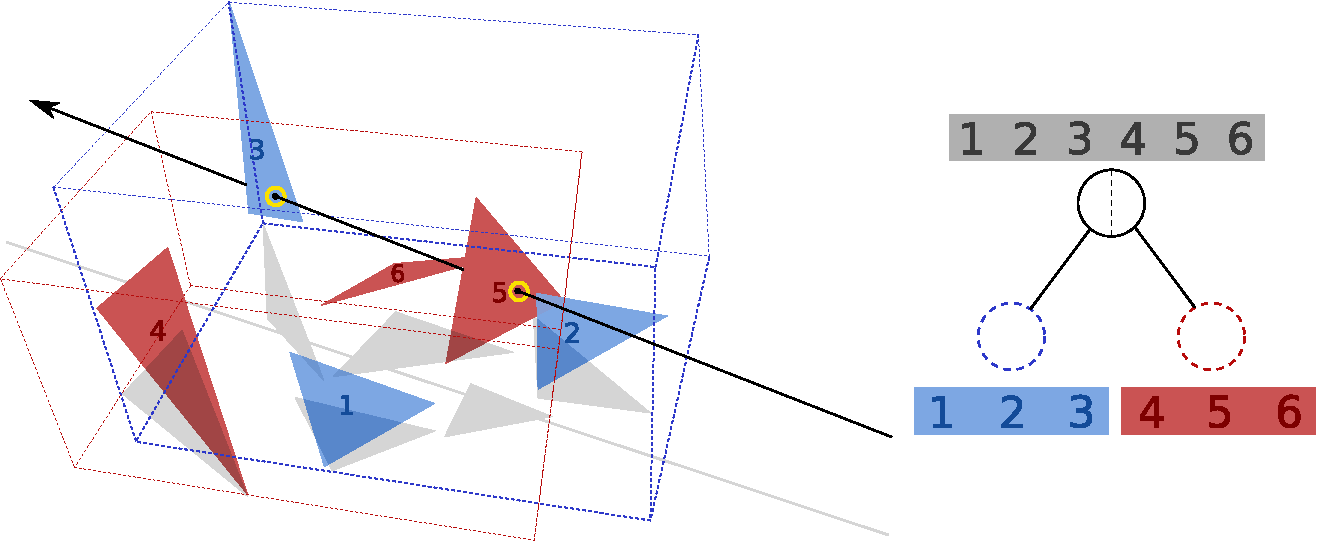
\includegraphics[width=1.0\textwidth]{images/bvh.pdf} 
\caption[Keine frühe Terminierung für BVHs]{Wird nach Fund des Schnittpunkts im blauen Teilbaum, der rote Teilbaum nicht mehr besucht, wird der nächste, gesuchte Schnittpunkt überhaupt nicht gefunden.}
\label{fig:bvhoverlap}
\end{figure}

Wenn in dem Teilbaum dessen AABB zuerst vom Strahl geschnitten wird, ein Schnittpunkt gefunden wurde, muss deshalb auch der andere Teilbaum durchsucht werden.
Wird ein Schnittpunkt gefunden kann das Strahlsegment bis zum Schnittpunkt \textit{gekürzt} werden, da potentielle weitere Schnitte die hinter dem bereits gefundenen Schnittpunkt liegen, uninteressant sind. Dadurch muss ein Knoten dessen AABB hinter dem verkürzten Segment des Strahls beginnt, nicht mehr traversiert werden (siehe Abbildung \ref{fig:bvhearlyexit}

\begin{figure}\centering
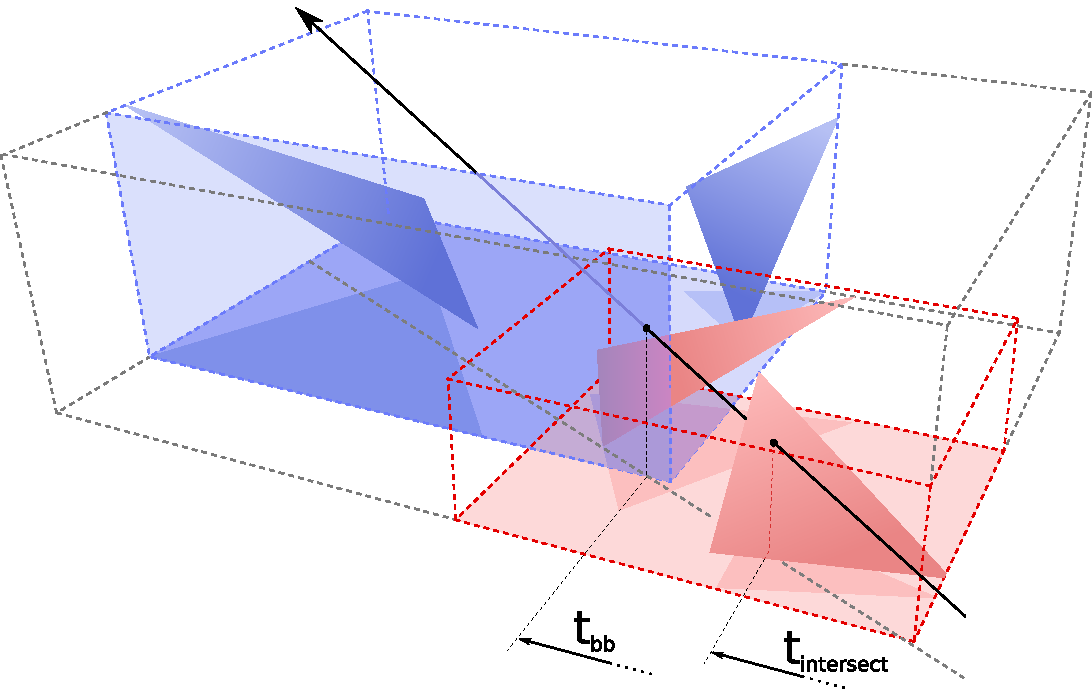
\includegraphics[width=0.7\textwidth]{images/bvhearlyexit.pdf} 
\caption[Begrenzung der Traversierung durch Verkürzen des Strahlsegments]{Da $t_{bb}$ größer ist als $t_{intersect}$ muss der Knoten zu dem die blaue AABB gehört nicht mehr traversiert werden. Der Strahl schneidet zwar die blaue AABB, das relevante Strahlsegment kann aber auf $t_{intersect}$ verkürzt werden.}
\label{fig:bvhearlyexit}
\end{figure}

In einem ersten systematischen Vergleich verschiedene Be"=schleu"=ni"=gungs"=strukturen (\cite{Havran00}) haben die kd-Trees wesentlich besser abgeschnitten als die BVHs. Dies ist zum Teil dadurch zu erklären, dass die frühzeitige Terminierung für BVHs nicht so strikt vorgenommen kann wie bei Verfahren, die den Raum disjunkt aufteilen. Ursache ist also die Überlappung der AABBs benachbarter Knoten.
Durch die fehlende Berücksichtigung der räumlichen Verteilung der Objekte bei der zuvor beschriebenen Konstruktion, kann eine beliebig große Überschneidung entstehen.
\cite{Havran00} wendet einen Konstruktionsalgorithmus von \cite{GoldsmithSalmon87} zur Bottom-Up Konstruktion der BVH an. Interessanterweise basiert die Entwicklung der SAH Kostenfunktionen auf Überlegungen aus \cite{GoldsmithSalmon87}.
Inzwischen haben \cite{WBS07} gezeigt, dass mit BVHs, durch die Konstruktion mit der SAH durchaus vergleichbare Ergebnisse zu kd-Tree basierten Systemen erreicht werden können.


\section{Hybride Raumaufteilung}

Um von den Stärken beider Vorgehensweisen zu profitieren wurden in letzter Zeit, unabhängig voneinander, mehrere ähnliche Verfahren entwickelt (unter anderem \cite{ZunigaUhlmann06}, \cite{HHS2006}) die versuchen die Vorteile von kd-Trees und BVHs zu kombinieren. Stellvertretend soll hier die Bounding Intervall Hierarchy(BIH)\abbrev{BIH}{Bounding Intervall Hierarchy} von \cite{BIH06} vorgestellt werden.

Anstatt eine komplette Bounding Box in jedem Knoten zu speichern, enthält ein innerer Knoten lediglich zwei, zu einer Hauptachse orthogonalen, Ebenen sowie Referenzen zu zwei Kindknoten.
\begin{lstlisting}[float,caption=Die Bounding Interval Hierarchy Inter Datenstruktur in erweiterter Backus-Naur-Form,label=bihdef]
 BIH        = InnerNode | Leaf
 InnerNode  = Axis float float BIH BIH
 Leaf       = { Primitiv }
\end{lstlisting}

Wächter schlägt zur Konstruktion eine neue, globale Heuristik vor. Dabei wird die AABB Szene für jeden Rekursionsschritt entlang der längsten Achse am räumlichen Median geteilt. Die Objekte werden dann jeweils danach, welchen der Subvoxel sie am meisten überlappen, in den rechten oder linken Teilbaum einsortiert. Für Dreiecke wird meistens lediglich geprüft ob der Schwerpunkt vor oder hinter der Trennebene liegt. Die beiden Ebenen werden anschließend auf die maximale beziehungsweise minimale Ausdehnung der Objekte im linken, beziehungsweise rechten Teilbaum, entlang der aktuellen Achse gesetzt.
Der Vorgang wird für die Teilmengen wiederholt bis lediglich ein Objekt in der Liste verbleibt, für welches dann ein Blattknoten angelegt wird. Wichtig ist, dass der Voxel dessen Mittelpunkt für die Bestimmung der Trennebene verwendet wird, nicht an die tatsächliche AABB der enthaltenen Objekte angepasst wird. Quelltext \ref{constrbih} veranschaulicht die Vorgehensweise.
\srcref{acceleration}{Bih}{construct}

\begin{lstlisting}[belowcaptionskip=8pt,float,mathescape=true,caption={[Konstruktion einer BIH mit globaler Heuristik]Konstruktion einer BIH mit der von Wächter vorgeschlagenen globalen Heuristik},label=constrbih]
BihNode subdivide(List<Primitive> primitives, AABB $aabb_{node}$, int depth) {
  if ( ( primitives.size() == 1 ) || ( depth == 0 ) ) 
    return new Leaf(primitives[0]); // create leaf

  $split_{axis}$ = $aabb_{node}$.getLongestAxis();
  $split_{pos}$ = $aabb_{node}.Min_{axis} + \frac{aabb_{node}.width_{axis}}{2}$;
  left = 0;
  right = primitives.size() - 1;
  do {// quicksortlike in-place partitioning
    while ( left < right && $primitives[left].center_{axis} <= split_{pos}$ ) 
      ++left;
    while ( right > left && $primitives[right].center_{axis} > split_{pos}$ )
      --right;
    if ( left < right ) 
      primitives.swap(left, right);
  } while ( left < right );

  if ( $primitives[right].center_{axis} < primitives[left].center_{axis}$ )
      primitives.swap(left, right);
  List<Primitive> leftPrimitives  = primitives.range(start, left - 1);
  List<Primitive> rightPrimitives = primitives.range(left, end);

  AABB leftBox = nodeAABB.split(axis, splitPos, left);
  AABB rightBox = nodeAABB.split(axis, splitPos, right);
  if ( left == end + 1 ) // all objects left
    return subdivide ( start, end, leftBox, depth );
  else if ( left == start ) // all objects right
     return subdivide ( start, end, rightBox, depth );
  else {
    leftMax = $nodeAABB.Min_{axis}$;
    rightMin = $nodeAABB.Max_{axis}$;
    foreach ( primitive in leftPrimitives )
        if ( $primitive.aabb.Max_{axis} > leftMax$ )
          leftMax = $primitive.aabb.Max_{axis}$;
    foreach ( primitive in rightPrimitives )
        if ( $primitive.aabb.Min_{axis} < rightMin$ )
          leftMax = $primitive.aabb.Min_{axis}$;
    return new Innernode( subdivide(leftPrimitives,  leftBox,  depth - 1 ), // left node
                          subdivide(rightPrimitives, rightBox, depth - 1),  // right node
                          leftMax, rightMin, axis);
  }
}
\end{lstlisting}

Da die Objekte nur in einen der beiden Kindknoten einsortiert werden, teilt sich die BIH mit der BVH die Vorteile, die durch die einmalige Referenzierung eines Objekts entstehen. Im Gegenzug kann es passieren, dass das Maximum der Objekte die vor der Trennebene liegen, größer ist als das Minimum der Objekte die hinter der Trennebene liegen. Damit teilt die BIH auch den Nachtteil der BVH, dass bei Fund eines Schnittpunkts, der Teil des Baums der noch nicht untersucht wurde, zumindest für den Bereich der Überlappung, noch traversiert werden muss. Durch die Quicksort-ähnliche Sortierung bei der Konstruktion wird jedoch sichergestellt, dass die Überlappung so klein wie möglich gehalten wird. Da wie bei der BVH Bereiche hinter dem gefundenen Schnittpunkt von der Suche ausgeschlossen werden können, werden die Fälle in denen beide Kindknoten traversiert müssen, auf ein Minimum reduziert.
Ein Knoten der BIH lässt sich fast so kompakt darstellen wie der eines kd-Trees, da im Gegensatz zur BVH nicht ganze AABBs gespeichert werden. Auch die Tests bei der Traversierung fallen ähnlich einfach wie bei den kd-Trees aus, da lediglich entlang einer Achse getestet werden muss. Dies ermöglicht auch die eindeutige Bestimmung der Traversierungsreihenfolge, wie sie bei kd-Trees vorgenommen wird. Quelltext \ref{travbih} zeigt wie einfach die Suche nach einem Schnittpunkt durchzuführen ist.
\srcref{acceleration}{Bih}{getFirstIntersection}

\begin{figure}\centering
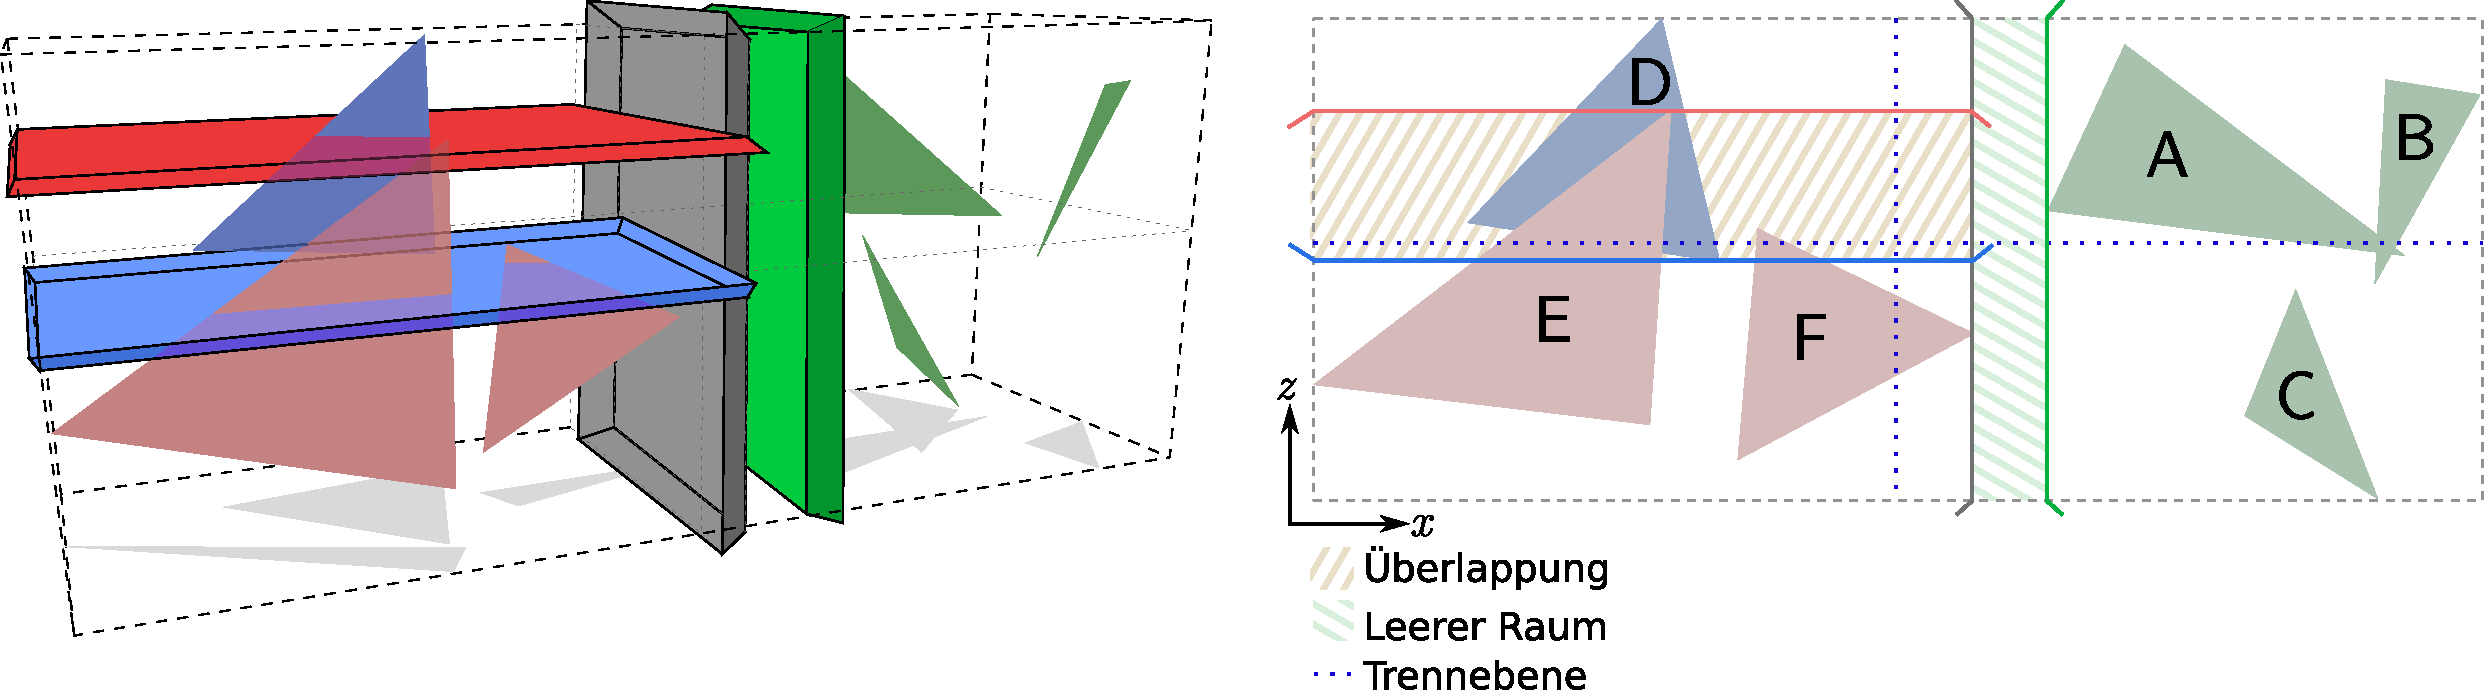
\includegraphics[width=1.0\textwidth]{images/bih.pdf} 
\caption[Beispiel für eine Raumaufteilung mit der BIH]{Beispiel für eine Raumaufteilung mit der BIH. Durch die erste (vertikale) Trennebene werden die Objeke A,B,C von den restlichen getrennt. Dabei entsteht keine Überlappung. In der nächsten Stufe wird das Dreieck D von den beiden anderen Dreiecken E und F in diesem Knoten getrennt. Dabei ergibt sich die eingezeichnete Überlappung, da das Maximum des Knotens der E und F enthält größer ist, als das Minimum des Knotens der D enthält.}
\label{fig:bih}
\end{figure}

\begin{lstlisting}[belowcaptionskip=8pt,float,mathescape=true,caption={[Traversierung der Bounding Interval Hierarchy]Traversierung der BIH. Der += Operator weißt nur dann zu wenn der rechte Operand einen kleineres t aufweist als der linke.},label=travbih]
Intersection searchClosestIntersection( BIH node, Ray ray, float $t_{min}$, float $t_{max}$ ) {
  Intersection closest(); // intialisiert mit dem 'leeren' Schnittpunkt
  if ( node.isLeaf() ) {
    foreach ( primitive in node.primitives  )
      closest += primitive.getIntersection( r );
    return closest;
  }
                                       // aus der Strahlrichtung kann geschlossen werden
  if ( r.direction[node.axis] > 0.0 ) {// welcher Kindknoten als erstes geschnitten wird
    ( near, far ) = ( left, right );
  else 
    ( near, far ) = ( right, left );

  $t_{near}$ = ( node.$plane_{near}$ - ray.origin[node.axis] ) / r.direction[node.axis];
  $t_{far}$   = ( node.$plane_{far}$ - ray.origin[node.axis] ) / r.direction[node.axis];

  if ( $t_{min}$ > $t_{near}$) { // naher voxel wird nicht vom Strahl geschnitteen
    if ( $t_{far}$ < $t_{max}$ ) { // entfernter Voxel wird geschnitten
      closest += searchClosestIntersection(node.$child_{far}$, ray, max( $t_{min}, t_{far}$), $t_{max}$);
    } // else: Strahl verlaueft zwischen Ebenen und schneidet keinen der Kindvoxel
  } else if ( $t_{far}$ > $t_{max}$) { // ausschliesslich der nahe Voxel muss durchsucht werden
    closest += searchClosestIntersection( node.$child_{near}$, ray, $t_{min}$, min( $t_{max}$, $t_{near}$ ));
  } else { // beide Knoten muessen durchsucht werden
    closest += searchClosestIntersection( node.$child_{near}$, ray, $t_{min}$, min($t_{max}$, $t_{near}$ ));
    closest += 
      searchClosestIntersection( node.$child_{far}$, ray, max($t_{min}$, $t_{far}$), min(closest.t , $t_{max}$));
  }
  return closest;
}
\end{lstlisting}

\section{Paket- und Frustumtraversierung}
\label{sec:packets}
Eine weitere Klasse von Verfahren, die sich mit den bisher beschriebenen Datenstrukturen kombinieren lässt, nutzt die räumliche Kohärenz von Strahlen aus. Darunter versteht man praktisch, Strahlen deren Ursprünge nah beieinander liegen und die sich in ähliche Richtungen ausbreiten. Diese Form der Kohärenz tritt besonders für \textit{Primärstrahlen} auf, lässt sich bei geschickter Anordnung aber auch bei Sekundärstrahlen begrenzt ausnutzen.

Das Verfahren profitiert von Fällen in denen viele Operationen, für alle Strahlen einer Gruppe das gleiche Ergebnis liefern. Genutzt werden hierfür konservative Tests die für ein Stellvertreter der Gruppe beantwortet werden, und durch dessen Eigenschaften die Ergebnisse der Tests auf alle Strahlen der Gruppe verallgemeinert werden können.

\cite{DHS04} wenden diese Idee das erste Mal für den Schnittest von Strahlpaketen mit Dreiecken an. Anstatt jeden Strahl einzeln mit dem Dreieck zu testen, werden zunächst die vier ``Eckstrahlen'' jeweils den folgenden fünf Tests unterzogen:
\begin{enumerate}
 \item liegt die Ebene des Dreiecks vor Beginn des Strahlsegments ($t_{split} < t_{min}$)
 \item liegt die Ebene des Dreiecks nach Ende des Strahlsegments ($t_{split} > t_{max}$)
 \item für jede der \textbf{drei} baryzentrischen Koordinaten des Schnittpunktes von Strahl und Ebene des Dreiecks wird getestet ob diese negativ ist (zu baryzentrischen Koordinaten siehe \ref{sec:barycentric}).
\end{enumerate}

\begin{figure}\centering
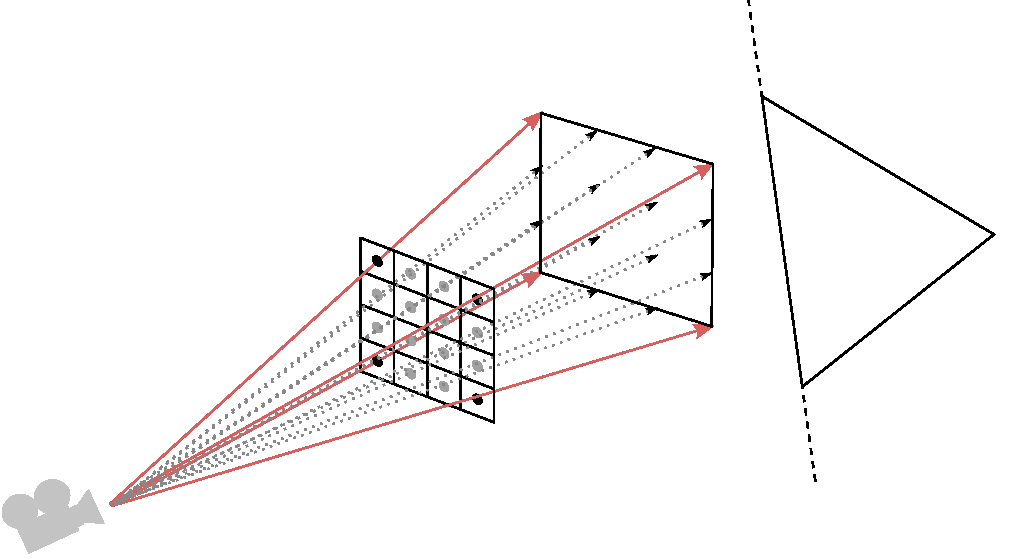
\includegraphics[width=0.7\textwidth]{images/packetmisstri.pdf} 
\caption[Früher Ausschluss ganzer Strahlpakete]{Die Schnittpunkte der vier Eckstrahlen liegen außerhalb der gleichen Seite des Dreiecks (eine baryzentrische Koordinate muss außerhalb von $[0,1]$ liegen siehe Anhang \ref{sec:barycentric}). Durch die Konvexität des Vierecks kann geschlossen werden, dass auch die ``inneren'' Strahlen keinen gemeinsamen Punkt mit dem Dreieck besitzen.}
\label{fig:packetdismiss}
\end{figure}

Schlägt einer dieser Tests für alle vier ``Eckstrahlen'' gleichzeitig fehl, verfehlt das gesamte Paket das Dreieck. Durch die Konvexität des Pyramidenstumpfes, der durch die vier Eckstrahlen gebildet wird, kann direkt geschlossen werden, dass keiner der Strahlen in dem Paket das Dreieck schneidet (siehe Abbildung \ref{fig:packetdismiss}).
Für die Fälle, in denen keiner der Tests für alle vier Strahlen gleichzeitig fehlschlägt, muss der Test jedoch für alle Strahlen des Pakets einzeln durchgeführt werden.

Die Kohärenz lässt sich nicht nur bei den Schnitttests von Strahlen und Dreiecken anwenden, sondern kann bereits bei der Traversierung der Beschleunigungsdatenstruktur ausgenutzt werden. Für kohärente Strahlen werden während der Traversierung ähnliche Teile der Beschleunigungsdatenstruktur besucht. Die Operationen die dabei durchgeführt werden müssen, können dabei für die Strahlen im Paket zusammengefasst und somit effizienter ausgeführt werden.

Die Traversierungsroutine der Raumaufteilungsverfahren muss allgmein wie folgt angepasst werden  um die Verarbeitung von Strahlpaketen zu ermöglichen. Bei den beschriebenen Verfahren wurde bisher für einen einzelnen Strahl festgestellt welche Voxel von diesem Strahl geschnitten werden. Für Pakete von Strahlen können für die im Paket enthaltenen Strahlen unterschiedliche Voxel geschnitten werden (siehe Abbildung \ref{fig:packettraversal}). Die Untersuchung muss deshalb für \textbf{jeden} der Voxel die von \textit{irgendeinem} Strahl des Pakets geschnitten werden, für das gesamte Paket fortgesetzt werden.

\begin{figure}\centering
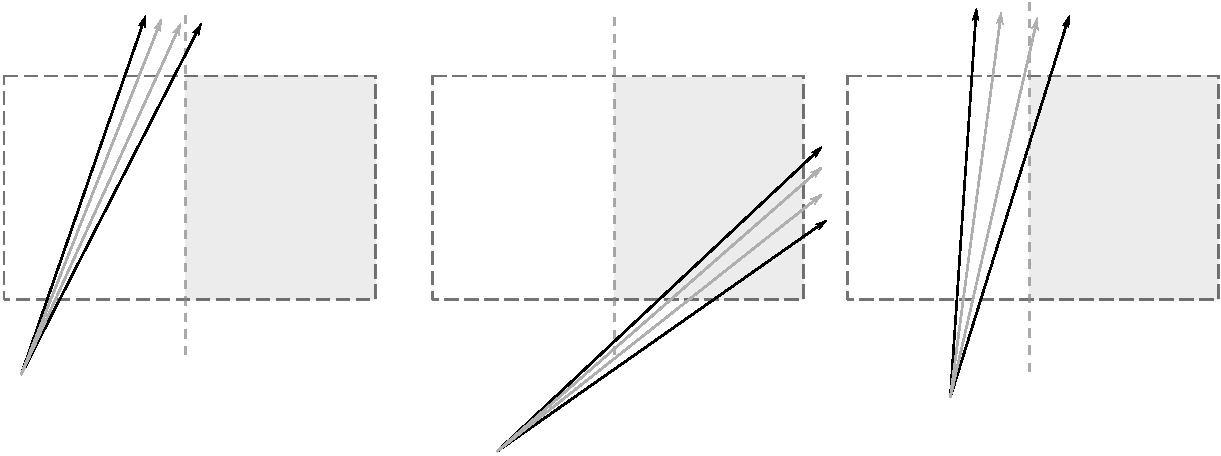
\includegraphics[width=0.7\textwidth]{images/packettraversal.pdf} 
\caption[Verfolgung von Strahlpaketen am Beispiel kd-Tree]{Verfolgung von Strahlpaketen am Beispiel kd-Tree. links: alle Strahlen schneiden lediglich den linken Voxel, die Traversierung wird lediglich für den linken Teilbaum fortgesetzt. mitte: die Traversierung muss lediglich für den rechten Teilbaum fortgesetzt werden. rechts: sobald auch nur ein Strahl des Pakets einen Voxel schneidet muss dieser Voxel untersucht werden. Deswegen müssen hier beide Teilbäume traversiert werden.}
\label{fig:packettraversal}
\end{figure}

Dadurch, dass Knoten auch besucht werden, wenn sie lediglich von wenigen Strahlen des Pakets geschnitten werden, entsteht ein entsprechender Overhead. Dieser amortisiert sich allerdings für kohärente Pakete mit dem Leistungsgewinn, der durch die gemeinsame Traversierung entsteht. Der Leistungsgewinn wird erzielt indem nicht für jeden Strahl einzeln ermittelt wird welcher Voxel geschnitten wird. Vielmehr wird wieder über einen konvexen Stellvertreter für das gesamte Paket ermittelt welche Voxel potentiell geschnitten werden. So lassen sich schnell ganze Teilbäume verwerfen.
Dieser Ansatz ist für jedes Raumaufteilungsverfahren einsetzbar. Die effiziente Implementierung unterscheidet sich aber für die verschiedenen Verfahren stark und wird deshalb für die in Kapitel \ref{sec:introstructs} vorgestellten Strukturen nachfolgend kurz dargestellt.



\subsection{Pakettraversierung für reguläre Gitter}
\begin{figure}\centering
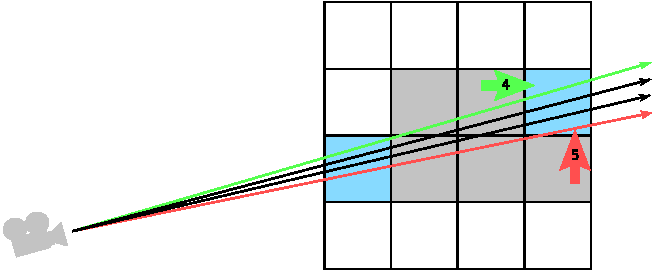
\includegraphics[width=0.5\textwidth]{images/gridpacket.pdf} 
\caption[Probleme bei Verfolgung von Strahlpaketen in regulärem Gitter (2D)]{Probleme bei Verfolgung von Strahlpaketen in regulärem Gitter (2D). Durch die gleichmäßig ``feine'' Aufteilung divergieren die Strahlen schneller als bei hierarchischen Strukturen. Das Strahlpaket könnte zwar aufgeteilt werden, jedoch werden unter Umständen wieder die gleichen Zellen besucht. Man könnte die Pakete dann natürlich wieder zusammenfügen. Zusätzlich kann die Zelle jedoch nach unterschiedlich vielen Schritten von den verschiedenen Paketen besucht werden, was dieses Vorgehen insgesamt unattraktiv macht.}
\label{fig:divergeandcommon}
\end{figure}


\cite{WIKKP06} haben, bereits mit dem Anspruch animierte Szenen darzustellen, einen effizienten Algorithmus zu Verfolgung kohärenter Strahlpakete durch gelichmäßige Gitter präsentiert. Um der in Abbildung \ref{fig:divergeandcommon} dargestellten Problematik aus dem Weg zu gehen, wird, anstatt das in \ref{sec:grids} vorgestellte Verfahren zu erweitern wird, ein komplett neuer Ansatz gewählt.

Zunächst muss für das Paket eine der Achsen des Weltkoordinatensystems als \textit{Hauptachse} $k$ gewählt werden. Entlang dieser müssen sich von den Strahlen im Paket entweder alle in positiver oder alle in negativer Richtung ausbreiten. Dies stellt keine Einschränkung für \textit{kohärente} Pakete dar, da für den Fall das dies nicht gegeben wäre, zwischen zwei Strahlen ein Winkel größer als 180° aufgespannt würde - was nicht mehr dem Kohärenzkritierum entspräche. Die beiden verbleibenden Achsen werden mit $u$ und $v$ bezeichnet.

\begin{figure}\centering
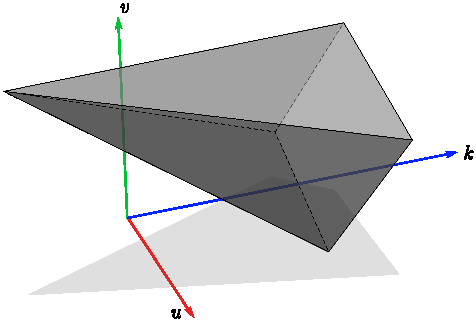
\includegraphics[width=0.5\textwidth]{images/gridmainaxis.pdf} 
\caption[Gemeinsame Hauptachse für scheibenbasierte Gittertraversierung]{Für die scheibenbasierte Gittertraversierung wird eine Hauptachse $k$ bestimmt entlang derer sich alle Strahlen eines Paketes in gleicher Richtung ausbreiten (positiver bzw. negativer). }
\label{fig:gridmainaxis}
\end{figure}

\cite{WIKKP06} schlagen nun vor das Gitter in Scheiben zu analysieren. Eine Scheibe des Gitters bilden dabei alle  Gittervoxel für die der Gitterindex entlang $k$ den gleichen Wert hat. Das Verfahren beginnt mit der ersten Scheibe, die von dem Strahlpaket geschnitten wird. Für die Scheibe wird ermittelt welche der enthaltenen Voxel von mindestens einem Strahl geschnitten werden. Die Objekte dieser Voxel werden dann mit jedem Strahl auf Schnitt getestet. Danach wird mit der nächsten Scheibe in Richtung $k$ ebenso fortgefahren. Der Vorteil im Vergleich zur der Vorgehensweise nach Abschnitt \ref{sec:grids} ist, dass das Strahlpaket nun immer als Ganzes behandelt werden kann. Andererseits führt es aber auch dazu, dass Strahlen mit Objekten geschnitten werden, deren Voxel sie nicht schneiden. Die zusätzlichen Kosten amortisieren sich jedoch für kohärente Pakete über das gesamte Verfahren.
Mit dieser Grundlage kann man nun dazu übergehen, die Überlappung der Strahlen und einer Gitterscheibe nicht mehr per Strahl vorzunehmen. Anstatt dessen wird die konvexe Hülle des Strahlpakets in Form eines Pyramidenstumpfs ermittelt. Im einfachsten Fall - für Primärstrahlen eines Rechtecks im Bildbereich - sind dies einfach die vier Eck-Strahlen eines Bündels.
Die Überlappung des Pyramidenstumpfs wird vereinfacht als achsenparallels Rechteck dargestellt (siehe \ref{fig:gridslices} c)).
Die aktuelle Ausbreitung dieses Rechtecks pro Scheibe, kann iterativ durch die Addition der zuvor ermittelten Steigungen (${\Delta{u}}_+, {\Delta{u}}_-, {\Delta{v}}_+, {\Delta{v}}_-$) errechnet werden (siehe Abbildung \ref{fig:gridslices} b) ${\Delta{u}}_+, {\Delta{u}}_-$).
Die Umwandlung der so errechneten Werte in Gitterindizes erhält man durch Subtraktion der Werte vom Gitterursprung und anschließende Division durch die Breite eines Voxels.

\begin{figure}\centering
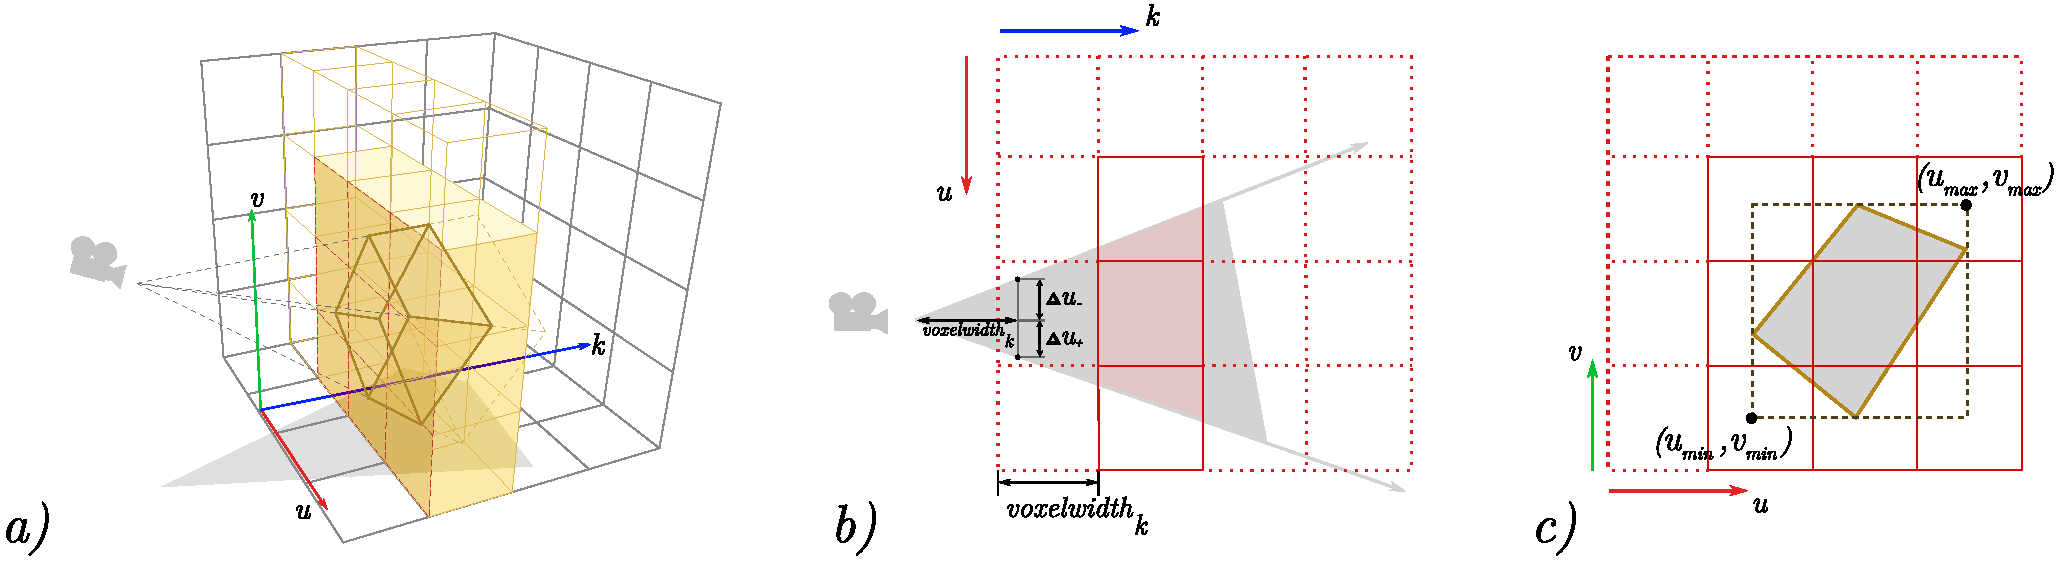
\includegraphics[width=1.0\textwidth]{images/gridslices.pdf} 
\caption[Scheibenbasierte Gittertraversierung]{a) Für die Traversierung sind lediglich die Voxel einer Scheibe interessant, die von dem Pyramidenstumpf geschnitten werden b) Durch die Seiten des Pyramidenstumpfs lässt sich bestimmen um wieviel sich der Ausschnitt einer Scheibe der die relevanten Voxel enthält pro Schritt in Richtung $k$ ausdehnt. c) Ausschnitt der aktuellen Scheibe in der Frontalansicht}
\label{fig:gridslices}
\end{figure}

Wie bereits in der Einführung zu disjunkten Raumaufteilungsverfahren erwähnt kann es bei regulären Gittern besonders für große Objekte dazu kommen, dass diese in mehreren Voxeln referenziert werden. Da durch die Regelmäßigkeit die Voxelgrenzen nicht an die Objekte angepasst werden, trifft dies auch für kleinere Objekte häufig zu und führt dazu, dass die meisten Objekte mehrfach referenziert werden. Durch die Traversierung von Paketen ergeben sich zusätzliche redundante Strahl-Objekt-Schnittests, da alle Strahlen immer gegen alle Objekte aller vom Paket geschnittenen Voxel einer Scheibe getestet werden. Deswegen profitiert die Pakettraversierung umso mehr von dem Einsatz von \textit{Mailboxing}. Der Overhead, der dabei pro Strahl entsteht, ist jedoch wesentlich geringer als bei der Traversierung einzelner Strahlen, da das \textit{Mailboxing} auf das ganze Paket angewendet werden kann. Konkret heißt das, dass die Objekte beim Schnittest mit einer \textit{Paket}-ID anstatt einer Strahl-ID gekennzeichnet werden. Trifft die Traversierung auf ein Objekt das bereits mit dem aktuellen Paket markiert wurde, kann der Test für alle Strahlen des Pakets übersprungen werden.\citep{WIKKP06}

\subsection{kd-Trees}
\label{sec:kdpacket}
Der Traversierungsalgorithmus für kd-Trees kann recht intuitiv für die Verarbeitung von Strahlpaketen angepasst werden. Die Entscheidung, ob an einem inneren Knoten mit dem linken, dem rechten oder beiden Teilbäumen fortgefahren wird, hängt nun lediglich davon ab, ob es \textit{irgendeinen} Strahl im Paket gibt, der den entsprechenden Subvoxel schneidet. An den Blattknoten werden alle Strahlen des Pakets mit den enthaltenen Objekten auf Schnitt getestet.
Einer der Gründe warum die kd-Trees die anderen Verfahren in vielen Fällen übertreffen ist die Möglichkeit die Objekte, die dem Strahlursprung näher gelegen, sind vor Objekten zu testen, die vom Ursprung weiter entfernt liegen. Deswegen kann die Suche entsprechend früher terminiert werden als bei anderen Verfahren. Hierfür ist aber die Befolgung der richtigen Traversierungsreihenfolge notwendig.
\cite{Wald04} und \cite{Benthin06} zeigen, dass eine eindeutige Bestimmung in welcher Reihenfolge die Kinder eines Knotens traversiert werden müssen für zwei allgemeine Fälle für Strahlpakete möglich ist. Abbildung \ref{fig:traversalorder} veranschaulicht, dass für den ersten Fall alle Strahlen den gleichen Ursprung besitzen müssen. Für den zweiten Fall müssen die Komponenten der Richtungsvektoren der verschiedenen Strahlen das gleiche Vorzeichen besitzen. Die eindeutige Reihenfolge bedeutet \textit{nicht}, dass jeder der Subvoxel von jedem tatsächlich Strahl getroffen wird. Es bedeutet lediglich, dass die Anwendung der frühen Terminierung in dieser Reihenfolge kein falsches Ergebnis liefert. Würde die Reihenfolge für die in Abbildung \ref{fig:traversalorder} schwarz eingezeichneten Strahlen auf die roten Strahlen angewandt und im als \textit{nah} markierten Knoten ein Schnittpunkt gefunden, würde bei der frühen Terminierung die Suche nach dem Besuch des ersten Kindknotens abgebrochen. Ein Schnittpunkt der in dem, für den roten Strahl fälschlicherweise als \textit{fern} markierten Knoten liegen würde, könnte nicht mehr gefunden werden.

\cite{Wald04} wählt als Kriterium die Gleichheit der Vorzeichen der Komponenten der Richtungsvektoren. Pakete die dieses Kriterium nicht erfüllen müssen gesondert behandelt werden. Am einfachsten lässt sich dies durch einzelne Verfolgung der Strahlen des Pakets umsetzen. Für kohärente Pakete tritt dieser Fall jedoch sehr selten ein.
Durch die Sicherheit, dass die Komponenten unterschiedlicher Richtungsvektoren das selbe Vorzeichen haben, lässt sich ein effizienterer Algorithmus zur Bestimmung der Reihenfolge finden als für den Fall, dass lediglich der Ursprung der Strahlen übereinstimmt. Da dieser Teil des Programms weitaus häufiger ausgeführt wird als eine anfängliche Überprüfung der Vorzeichen, ist die Vorzeichengleichheit als Kriterium dem des gleichen Ursprungs vorzuziehen.

\begin{figure}\centering
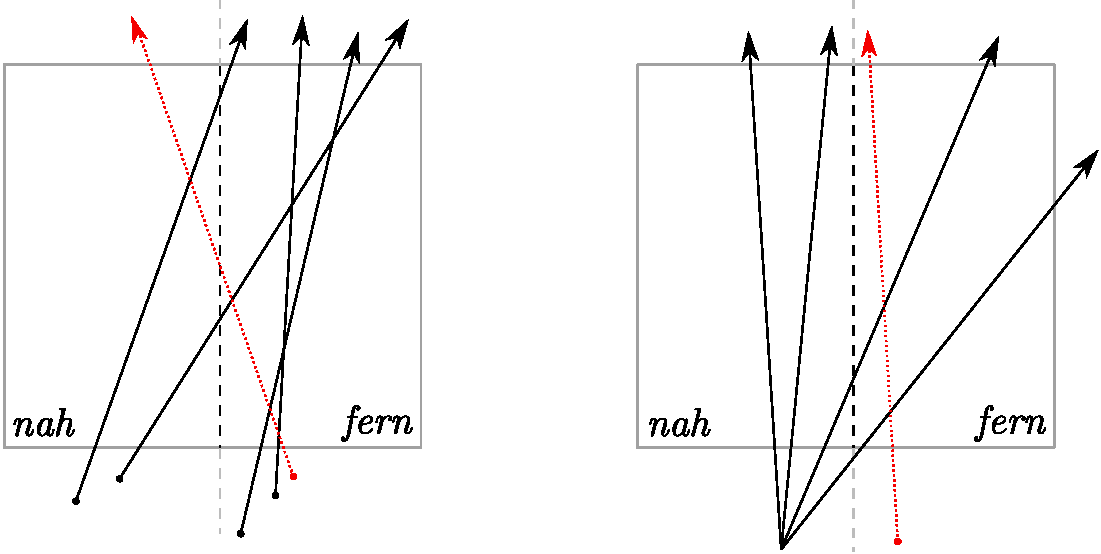
\includegraphics[width=0.65\textwidth]{images/traversalorder.pdf} 
\caption[Bestimmung der Traversierungsreihenfolge für Strahlpakete]{Bestimmung der Traversierungsreihenfolge. Der rote Fall bricht das jeweilige Kriterium, um zu zeigen, dass dies die Eindeutigkeit zerstört. links: Die Ausbreitungsrichtung ist für alle Strahlen entlang der Trennachse gleich. rechts: Der gleiche Ursprung ermöglicht die eindeutige Bestimmung der Reihenfolge.  }
\label{fig:traversalorder}
\end{figure}

\subsection{Bounding Volume Hierarchies}

\cite{WBS07} haben unter anderem ein effizientes Vorgehen zur Traversierung von BVHs entwickelt. Dabei werden verschiedene konservative Tests angewendet, um einfache Fälle während der Traversierung besonders schnell entscheiden zu können.

Der erste Test profitiert davon, dass ein Teilbaum durchsucht werden muss sobald einer der Strahlen im Paket die entsprechende AABB schneidet. Während der Traversierung wird für jeden Knoten verfolgt, welches der erste Strahl im Paket ist, der die AABB des Knotens schneidet. Dieser Strahl wird dann auch als erstes mit den Kindknoten auf Schnitt getestet.
So kann in vielen Fällen schnell entschieden werden, dass ein Kindknoten besucht werden muss. Trifft dieser Strahl nicht, werden nicht die restlichen Strahlen getestet sondern, zunächst der folgende Test ausgeführt.

Der zweite, so genannte ``early miss''-Test, prüft anhand von Intervallarithmetik, ob das Paket die AABB des Teilbaums überlappen kann. Ist dies ausgeschlossen, kann der Teilbaum ohne weitere Tests verworfen werden.

Hat keiner der beiden Tests ein positives Ergebnis geliefert, werden die restlichen Strahlen im Paket auf Schnitt mit der AABB des Teilbaums getestet bis entweder ein Strahl gefunden wird der sie schneidet oder für alle Strahlen festgestellt wird, dass sie die AABB verfehlen.

\subsection{Sekundärstrahlen}

Für die Schattenstrahlen der Schnittpunkte eines Strahlpakets lässt sich einfach ein kohärentes Strahlpaket finden indem die Schattenstrahlen umgedreht werden. Für den gemeinsamen Ursprung der Strahlen wird die Position der Lichtquelle gewählt. Die Richtungen der Schattenstrahlen zeigen auf die gefundenen Schnittpunkte. Die Kohärenz bleibt auch erhalten, wenn die Primärstrahlen nicht das selbe Objekt treffen, kann aber zerstört werden, wenn die Objekte weit voneinander entfernt liegen.
Für reflektierte Strahlen ist die Situation komplizierter. Kohärente Pakete von reflektierten Strahlen lassen sich effizient nur für solche Pakete finden, deren Strahlen an der gleichen Ebene reflektiert werden. Abbildung \ref{fig:secondaryrays} zeigt die entsprechenden Fälle.\citep{DHS04}
\begin{figure}\centering
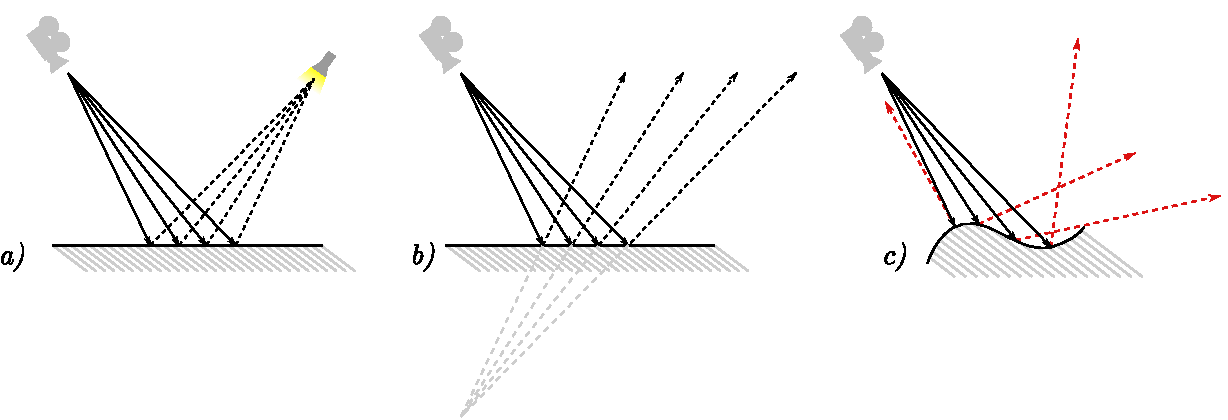
\includegraphics[width=0.9\textwidth]{images/secondaryrays.pdf} 
\caption[Kohärenz bei Sekundärstrahlen]{a) Erzeugung eines kohärenten Schattenstrahlpakets durch Verlagerung des Ursprungs zur Position der Lichtquelle. b) Bei Reflexion an einer ebenen Fläche bleibt die Kohärenz auch für die reflektierten Strahlen erhalten. c) Durch Reflexion an einer gekrümmten Fläche wird die Kohärenz der reflektierten Strahlen zerstört.}
\label{fig:secondaryrays}
\end{figure}

\chapter{Animation}

Kamerafahrten durch statische Modelle sind per Raytracing schon seit ein paar Jahren, auch auf Arbeitsplatzrechnern, möglich. Für animierte, beziehungsweise allgemein dynamische Szenen, müssen die verwendeten Algorithmen jedoch unter einem weiteren Aspekt betrachtet werden. Da sich die Geometrie hier von Frame zu Frame verändert, kann die für die vorherige Ausprägung der Geometrie erstellte Beschleunigungsdatenstruktur nicht mehr verwendet werden. Veränderte Positionen oder neue Objekte machen die Aussagen, die eine \textit{veraltete} Beschleunigungsstruktur trifft, ungültig.

\section{Klassifizierung von Problemen dynamischer Szene}

Für die Darstellung dynamischer Szenen müssen die bisher beschriebenen Datenstrukturen neu bewertet werden. \cite{BART} haben verschiedene Problemklassen für das Raytracing definiert:

\begin{enumerate}
  \item Hierarchische Animation
  \item Unstrukturierte Bewegung von Objekten
  \item ``Teapot-in-Stadium''-Problem
  \item Niedrige Kohärenz zwischen zwei Bildern
  \item Überlappende Bounding Volumen
  \item Variierende Objektverteilung
\end{enumerate}

Für dynamische Szenen besonders interessant sind die Punkte 1, 2 und 4. Die anderen Punkte treten auch für statische Szenen auf, durch die lediglich die Kamera bewegt wird. Deswegen werden nun diese drei Punkte näher erläutert.

\begin{description}
 \item[Hierarchische Animation] Bei der Animation, beziehungsweise Simulation von komplexen Bewegungen werden einzelne Teile hierarchischer Objekte häufig in einem lokalen Koordinatensystem modelliert. Anschließend wird dieses relativ zu dem Vorgängerknoten in einem Szenengraphen positioniert. Die einzelnen Teile ändern ihre Geometrie häufig über die gesamte Dauer der Animation nicht. Diese Art der Kohärenz kann ausgenutzt werden, um dynamische Szenen effizienter darzustellen. Allerdings werden Systeme, die hauptsächliche auf dieser Annahme aufbauen in Szenen mit einem kleinen Anteil hierarchischer Animation dementsprechend schwache Leistung zeigen
\item[Unstrukturierte Bewegung] Bei der unstrukturierten Bewegung gibt es keinerlei Zusammenhang zwischen den Bewegungen einzelner Objekte. Da keine Kohärenzen zwischen den Objekten ausgenutzt werden können stellt dies ein komplexes Problem für jeden Raytracer dar.
\item[Niedrige Kohärenz zwischen zwei Frames] Ähneln sich zwei aufeinanderfolgende Bilder, können unter Umständen Informationen aus dem letzten Bild verwendet werden, um das aktuelle schneller zu berechnen. Dies gilt sowohl für Algorithmen, die dies im Bildbereich ausnutzen als auch für die Position und Orientierung der 3D-Objekte im Raum. Das Fehlen einer solchen Kohärenz kann entsprechende Verfahren verlangsamen.
 \end{description}

\section{Konsequenzen für die Datenstrukturen}

Der einfachste Ansatz Veränderungen der Szenengeometrie zu berücksichtigen ist der komplette Neuaufbau der Beschleunigungsdatenstruktur für jedes Frame. Die Konstruktionszeiten variieren sehr stark. Sie können je nach Datenstruktur, Heuristik und Anzahl der Objekte von ein paar Millisekunden bis zu einigen Minuten dauern.
Natürlich ist es wünschenswert, Strukturen die für das letzte Frame erstellt wurden soweit wie möglich weiterzuverwenden. Dies ist jedoch nicht für alle der beschriebenen Datenstrukturen uneingeschränkt möglich.


\subsection{Trennung von statischen und dynamischen Inhalten}

Für Anwendungen, bei denen große Teile der Geometrie statisch sind, kann es sich auszahlen dynamische und statische Inhalte getrennt zu verarbeiten. Unter Umständen kann es sich sogar lohnen weiter zwischen hierarchischer und unstrukturierter Bewegung zu unterscheiden.
Dabei stellt sich die Frage nach welchen Kriterien diese Unterscheidung vorgenommen wird. \cite{Wald04} überlässt diese Entscheidung der Anwendung, in der dynamischen Inhalte gesondert spezifiziert werden müssen.
Ein ähnliches Vorgehen wird auch für Verfahren, welche die Rendering-Pipeline der Grafikkarte verwenden genutzt.So genannte  \textit{Vertex Buffer Objects} werden verwendet, um Geometriedaten direkt in den Grafikkartenspeicher zu schreiben. Dies kann genutzt werden, um die Darstellung von Inhalten die sich gar nicht oder nur sehr langsam ändern effizienter zu gestalten \cite{NVIDIA03}.

In \cite{GU06} wird die Möglichkeit aufgezeigt, durch Analyse von animierten Modellen in verschiedenen \textit{Posen}, Inhalte, die ausschließlich affiner Transformation unterzogen werden, automatisch zu identifizieren.

Für große Teile einer Szene, die lediglich als ganzes, affin transformiert werden, lohnt es sich die Beschleunigungsdatenstruktur getrennt aufzubauen. Pro Bild muss dann lediglich eine Datenstruktur aufgebaut werden, in der die Teilmodelle als ganze Objekte behandelt werden. Anstatt jedes Element der Teilmodelle in das Weltkoordinatensystem zu transformieren, wird zur Laufzeit lediglich der Strahl in das lokale Koordinatensystem des entsprechenden Modellteils transformiert. So kann ein großer Teil der Konstruktionszeit gespart werden.

Der Ansatz den Strahl in das Koordinatensystem von Modellteilen zu transformieren hat den positiven Nebeneffekt, dass sich die Teilgeometrien leicht \textit{instanziieren} lassen. Das heißt, die für ein Teilmodell aufgebaute Beschleunigungshierarchie kann an mehreren Knoten der \textit{``Meta''}-Struktur in Kobination mit weiteren Transformationen referenziert werden. Dies ist besonders effizient für Modelle in denen bestimmte Teilmodelle sehr häufig verwendet werden, da die Beschleunigungshierarchie für diese Teile nur einmal konstruiert und gespeichert werden muss. Wird der Strahl durch die Kaskadierung von Modellen jedoch häufig transformiert kann es durch die eingeschränkte Genauigkeit der Gleitkommaarithmetik zu numerischen bedingten Fehlern kommen.

\subsection{Aktualisierung von Beschleunigungsstrukturen}

Dennoch gibt es Fälle in denen keine oder zu wenig Informationen über die Dynamik der dargestellten Objekte zur Verfügung steht. Im Gegensatz zu den kd-Trees kann eine BVH aktualisiert werden ohne dass die Topologie verändert werden muss. Da die Topologie der BVH keine Aussage über die räumliche Verteilung der Objekte trifft, müssen nach einer Bewegung der Szenenobjekte lediglich die in den Knoten gespeicherten AABBs den neuen Ausdehnungen angepasst werden.
In den meisten Fällen führt dies mittelfristig jedoch zu einer Verschlechterung der Qualität der BVH. Die Strahlanfragen werden immer langsamer, je weiter die Animation fortschreitet. Entfernen sich Objekte, die einen gemeinsamen Vorgängerknoten besitzen, voneinander, vergrößern sie dessen AABB-Volumen und erhöhen somit die Anzahl der Strahlen für die dieser Knoten durchsucht werden muss (siehe Abbildung \ref{fig:bvhdegrade}).
Wie stark die Qualität der BVH nachlässt kann von vielen Faktoren abhängen (Ausprägung der Geometrie zu Konstruktionszeit, Heuristik, Ausprägung der Dynamik).
Um eine für die \textit{Deformierung} geeignete Anfangspartitionierung zu finden, beschreiben \cite{WBS07} die Analyse der Animation in verschiedenen Posen (zum Beispiel für Menschmodell). Dadurch lässt sich feststellen welche Objekte für die Dauer der Animation eine räumliche Nähe beibehalten. Dieses Vorgehen erfordert aber auch wieder entsprechendes Vorwissen über die Animation.

Völlig ohne Vorwissen über die Struktur und Bewegung der zugrundeliegenden Geometrie kommt das Verfahren von \cite{RTDEFORM} aus. Anhand einer Heuristik wird nach jeder Aktualisierung die Verschlechterung der Qualität der BVH gemessen. Überschreitet die Verschlechterung einen festgelegten Schwellwert wird die BVH neu aufgebaut. Die Heuristik misst die Größenänderung der Oberfläche der AABB eines Knotens im Vergelich zur Größenänderung der Oberflächen der AABBs der Kindknoten. So kann festgestellt wann sich die Oberfläche eines Knotens lediglich aufgrund der Verteilung der Objekte ändert. Fälle wie in Abbildung \ref{fig:bvhdegrade} können so frühzeitig festgestellt werden. Die BVH muss dann für die veränderte Objektverteilung neu konstruiert werden. Für Animationen in denen nur wenig Bewegung stattfindet wird unter Umständen kein Neuaufbau für die komplette Dauer nötig.
Das Verfahren wird leider nur für Szenen beschrieben, bei denen für die Dauer der Animation keine Objekte hinzugefügt oder entfernt werden. Eine entsprechende Anpassung kann jedoch nicht teurer sein als ein Neuaufbau der BVH und sollte dementsprechend einfach durchzuführen sein.

Die Aussagen und Verfahren, die hier über die Aktualisierung von BVHs vorgestellt wurden, sind auf alle anderen Verfahren, die auch die Objektliste partitionieren, wie zum Beispiel die BIH, direkt übertragbar.

\begin{figure}\centering
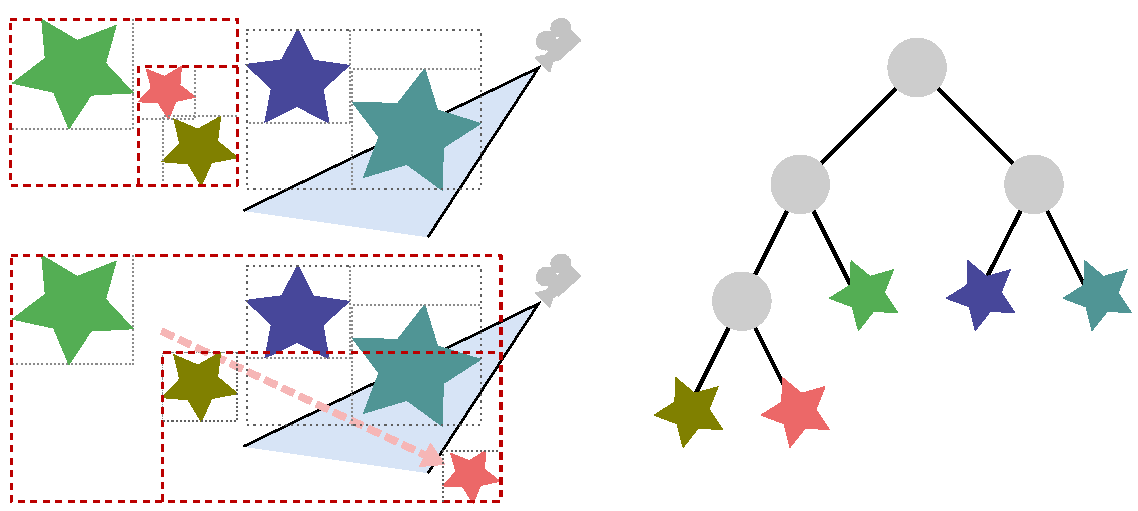
\includegraphics[width=1.0\textwidth]{images/bvhdegrade.pdf} 
\caption[Qualitätsverminderung einer BHV]{Qualitätsverminderung einer BHV. Bei Bewegung von Objekten kann die Topologie der BVH beibehalten werden, lediglich die BBs müssen angepasst werden. Doch durch ungünstige Bewegung, wie hier des roten Objekts, müssen für Strahlen des gezeigten Frustums alle inneren Knoten der BHV getestet werden. Ein Baum bei dem das rote Objekt im rechten Teilbaum der Wurzel einsortiert würde, wäre effizienter.}
\label{fig:bvhdegrade}
\end{figure}


\subsection{Schnelle Konstruktion}
\label{sec:lazy}
Trotz ausgereifter Verfahren zur Aktualisierung von BVHs stellt sich die Frage wie sich \textit{gute} Beschleunigungsdatenstrukturen möglichst effizient konstruieren lassen.
Ein Ansatz die Konstruktionszeit für hierarchische Datenstrukturen zu verringern ist es, die Datenstruktur vor der ersten Strahlanfrage gar nicht oder nur teilweise aufzubauen. Bei diesem \textit{lazy building} soll vermieden werden, dass Teile der Datenstruktur aufgebaut werden, die für das aktuelle Bild von keinem Strahl durchsucht werden müssen. Dies bietet sich besonders an, wenn zusätzlich die von der Anwendung bereitgestellten Daten vor der Konstruktion weiteren Vorverarbeitungsschritten unterzogen werden müssen (zum Beispiel die Tesselierung von Flächen\cite{RAZOR07}).
Die inneren Knoten der Datenstruktur müssen dafür um ein Datenfeld erweitert werden, welches darüber Auskunft gibt, ob die Teilbäume dieses Knotens für eine Strahlanfrage noch konstruiert werden müssen. Bei der Traversierung eines so markierten Knotens muss dann die Konstruktion der Teilbäume nachgeholt werden. Das verschiebt natürlich lediglich einen Teil des Konstruktionsaufwands in die Traversierungsphase. Teile der Hierarchie welche Objekte enthalten, die von keinem Strahl getroffen werden, müssen aber überhaupt nicht konstruiert werden. Abbildung \ref{fig:lazybuild} verdeutlicht wie dies für eine einfache Beispielszene aussehen könnte.
Für Verfahren, die ebenfalls Effekte globaler Beleuchtung darstellen, verringert sich der effektive Gewinn dieser Vorgehensweise unter Umständen jedoch drastisch. Da hier viele Teile der Szene untersucht werden müssen, obwohl sie von der Kameraposition direkt sichtbar sind, kann es passieren, dass doch nahezu der gesamte Baum der Beschleunigungsdatenstruktur aufgebaut werden muss.

\begin{figure}\centering
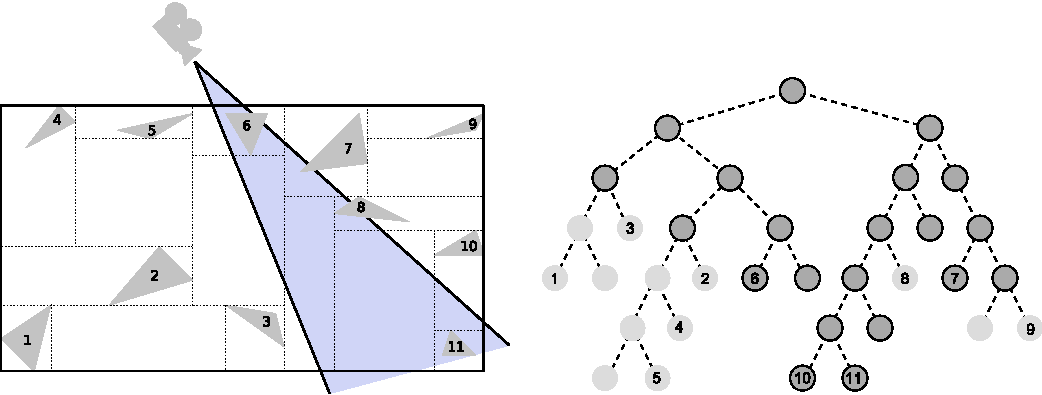
\includegraphics[width=1.0\textwidth]{images/lazybuild.pdf} 
\caption[Lazy build für binäre Raumaufteilung]{Binäre Raumaufteilung für eine sehr einfache Szene. Die hellen Knoten im Baum verursachen beim \textit{lazy build} keine Konstruktionskosten.}
\label{fig:lazybuild}
\end{figure}

Die Laufzeit des Konstruktionsalgorithmus hängt hauptsächlich von der Komplexität der Heuristik ab, die für die Partitionierung des Raums beziehungsweise der Objektmenge gewählt wird. Bei der Wahl der Heuristik geht es deshalb hauptsächlich darum, die höheren Kosten einer aufwändigen Heuristik in der Konstruktionsphase gegen die Beschleunigung der Strahlanfragen in der Traversierungsphase abzuwägen.

\subsubsection{SAH in  $O(N {log}^2 N )$}
\label{sec:nlog2n}
Die \textit{Surface Area Heuristic} nimmt momentan die beste Raumaufteilung vor. Der im letzten Kapitel beschriebene Ansatz zur Verwendung der SAH (\ref{perfectsplits}) bessitzt eine quadratische Komplexität in Abhängigkeit von den verwendeten Szenenobjekten und ist damit, außer für sehr kleine Szenen, nicht praktikabel.
Unter anderem in \cite{PBRT} wird vorgestellt wie man, ohne Beschränkung der Allgemeinheit, das Problem auch in $O(N {log}^2 N )$ lösen kann. Die Ursache für die quadratische Komplexität bei dem naiven Ansatz ist, dass die Anzahl der Objekte die sich auf der linken und rechten Seite einer potentiellen Schnittebene befinden ($N_{left}, N_{right}$) jedesmal durch Iteration über alle Objekte des Knotens ermittelt werden muss - und das für jeden Kandidaten der Trennebene in jedem inneren Knoten.

\begin{figure}\centering
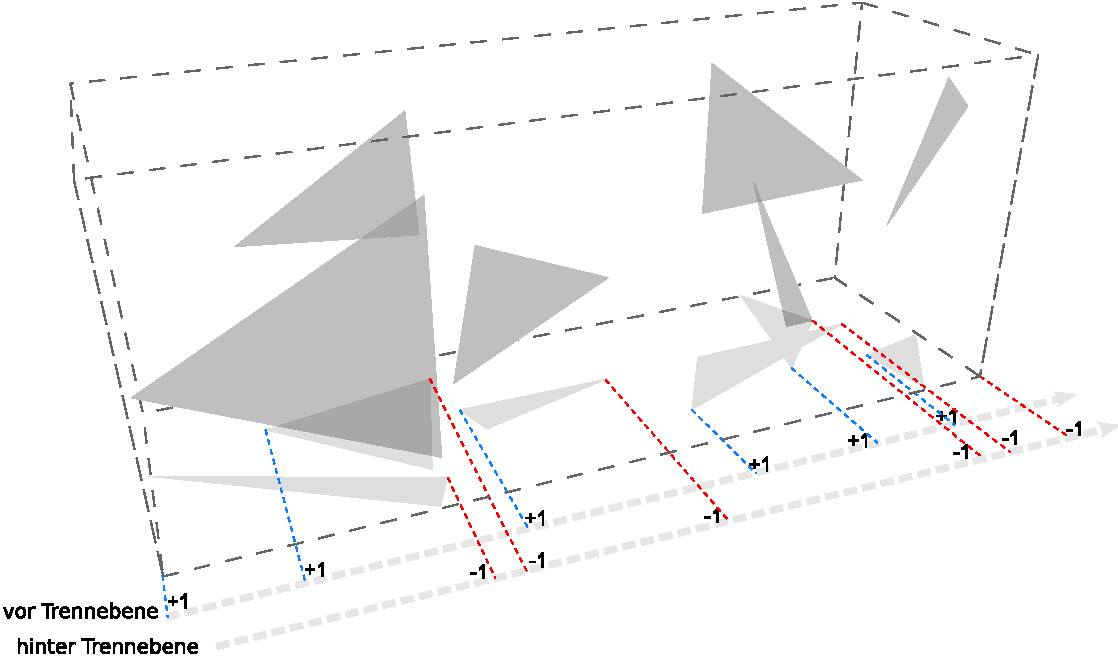
\includegraphics[width=0.7\textwidth]{images/splitevents.pdf} 
\caption[Inkrementelles Zählen der Objekte vor/hinter der Trennebene]{Durch zählen der bisher aufgetretenen Ereignisse lassen sich während der Iteration über die Liste die Objekte vor und nach dem aktuellen Ereignis bestimmen. Die Anzahl der Objekte vor der Ebene wird mit Null initialisiert und bei jedem ``Anfangs''-Ereignis(blau) inkrementiert. Die Anzahl der Objekte hinter der Ebene wird mit der Anzahl der Objekte in diesem Voxel initialisiert und bei jedem ``Ende''-Ereignis(rot) dekrementiert.}
\label{fig:splitevents}
\end{figure}

Um $N_{left}, N_{right}$ entlang einer Achse $k$ effizienter zu bestimmen, lässt sich die Tatsache nutzen, dass die Orte an denen sich diese Werte ändern mit den Positionen der potentiellen Schnittebenen zusammenfallen (nämlich die Minima/Maxima der AABBs der Objekte auf diese Achse). Die Stelle an der die AABB eines Objekts auf eine Achse beginnt oder endet wird auch ``Ereignis'' genannt.

\begin{lstlisting}[belowcaptionskip=12pt,float,mathescape=true,caption={[Definition des Ereignisdatentyps für die Kandidatengenerierung]Ereignisse bestehen aus einer Position $t$ und einer Kennzeichnung ob bei dieser Position ein Objekt beginnt oder endet. Für plane Objekte kann noch der Spezialfall eintreten, dass das Objekt komplett in eine Schnittebene an dieser Stelle fallen würde.},label=event]
Event     = float EventType
EventType = END | INPLANE | START 
\end{lstlisting}

Erstellt man eine sortierte Liste aller Ereignisse entlang einer Achse, lassen sich $N_{left}$, $N_{right}$ während einer Iteration über diese Liste durch einfaches ``Mitzählen'' bestimmen. Bei der Konstruktion der Ereignisliste wird zwischen Ereignissen bei denen eine AABB beginnt und denen, an denen sie endet unterschieden. Für plane Objekte muss zusätzlich der Fall berücksichtigt werden, dass ein Objekt komplett \textit{in} der Trennebene liegen kann. Abbildung \ref{fig:splitevents} veranschaulicht diesen Vorgang.
Um die Liste der Ereignisse sortieren zu können, muss auf den Ereignissen eine Ordnung definiert sein. Diese wird wie folgt definiert: $ (e_1 < e_2) = true$ wenn $e_1.t < e_2.t \lor ( (e_1.t = e_2.t) \land (e_1.type < e_2.type))$, wobei $t$ die Position des Ereignisses auf der aktuellen Achse darstellt. Für \verb|EventType| gilt wiederum: ${END} < {INPLANE} < {START}$.

Für die Evaluierung der Kandidaten werden alle Ereignisse, die an einer Stelle auftreten, ``aufgesammelt''. Durch die Ereignisse, die vor einer Stelle aufgetreten sind, kann auf die Anzahl der Objekte im linken, beziehungsweise rechten Subvoxel geschlossen werden. Plane Objekte, die parallel zur Trennebene liegen, benötigen eine gesonderte Behandlung. Liegt ein solches Objekt an der Stelle der Trennebene, und ist einer der beiden Subvoxel leer, ergibt sich ein besserer Baum, wenn diese Objekte in den nicht-leeren Teilbaum sortiert werden. Der komplette Algorithmus wird noch einmal in Quelltext \ref{sahnlog2n} in Pseudocode wiedergegeben.
\srcref{accelleration}{KdTreeSahNlog2N}{construct}

\begin{lstlisting}[belowcaptionskip=8pt,float,mathescape=true,caption={Algorithmus zur Bestimmung der besten Trennebene in  $O(N {log}^2 N )$},label=sahnlog2n,numbers=left]
(float, Axis) searchBestSplitPos(aabb voxel, List<Primitive> primitives) {
  ${axis}_{best} = {none}$
  ${candidate}_{best} = 0$
  ${cost}_{best} = \infty$
  foreach ( axis in {x,y,z} ) {
    List<Events> events;
    foreach (primitive in primitives)
      if ( primitive.aabb.min[axis] == aabb.max[axis] )
        events.add( Event(primitive.aabb.min[axis], INPLANE ) );
      else {
        events.add( Event(max(primitive.aabb.min[axis], voxel.min[axis]), START) )
        events.add( Event(min(primitive.aabb.max[axis], voxel.max[axis]), END) )
      }
    events.sort()
    $N_{left} = 0, N_{right} = event.length, N_{inPlane} = 0$
    event = events.first
    while( event in events ) {
        ${candidate}_{current}$ = event.t
        $p_{start} = p_{end} = p_{inPlane}$ = 0
        while( (event in events) && (event.t == ${candidate}_{current}$)
              && (event.t == END) ) {
          event = event.next
          ++$p_{end}$
        }
        while( (event in events) && (event.t == ${candidate}_{current}$)
              && (event.t == INPLANE) ) {
          event = event.next
          ++$p_{inPlane}$
        }
        while( (event in events) && (event.t == ${candidate}_{current}$)
              && (event.t == START) ) {
          event = event.next
          ++$p_{start}$
        }
        $N_{right} -= ( p_{end} + p_{inPlane} )$
        $N_{inPlane} = p_{inPlane}$
        ${cost}_{current}$ = SAH(v, ${candidate}_{current}$, axis, $N_{left}, N_{right}, N_{inPlane}$);
        if ( ${cost}_{current} < {cost}_{best}$ ) {
          ${cost}_{best} = {cost}_{current}$
          ${candidate}_{best} = {candidate}_{current}$
          ${axis}_{best} = axis$
        }
        $N_{left} += ( p_{start} + p_{inPlane} )$
        $N_{inPlane} = 0$
    }
  }
  return (${candidate}_{best}, {axis}_{best}$);
}


\end{lstlisting}

\subsubsection{SAH in $O(N {log} N)$}
\label{sec:nlogn}
Eine weitere Reduzierung der algorithmischen Komplexität der Konstruktion anhand der SAH gelang \cite{WaldHavran06}. Ihr Verfahren baut auf dem zuvor beschriebenen Prinzip auf. Sie vermeiden jedoch die erneute Sortierung der Ereignisliste. Anstatt dessen wird zu Beginn der Konstruktionsphase einmalig eine Liste aufgebaut, welche die Ereignisse entlang aller Achsen enthält. Jedes Ereignis muss nun zusätzlich um die Information erweitert werden auf welcher Achse es aufgetreten ist(siehe Abbildung \ref{fig:eventlist}). Außerdem wird für jedes Ereignis verfolgt, welches Objekt es ausgelöst hat.
Damit weiterhin eine Sortierung der Ereignisse möglich ist, muss auch die Ordnung auf den Ereignissen angepasst werden. Primäres Kriterium bleibt die Stelle an der das Ereignis auf einer der Achsen auftritt. Da aber für eine Stelle auf \emph{einer} Achse alle Ereignisse auf einmal ausgewertet werden sollen, wird als zweites Kriterium die Achse eingesetzt. Der Ereignistyp bleibt als letztes Kriterium. Sodas gilt $e_1 < e_2$ falls einer der folgenden Bedingungen erfüllt ist:
\begin{itemize}
 \item $e_1.t < e_2.t$
 \item $e_1.t = e_2.t \land e_1.axis < e_2.axis$
 \item $e_1.t = e_2.t \land e_1.axis = e_2.axis e_1.type < e_2.type$
\end{itemize}
Für eine effizientere Suche muss zunächst der Algorithmus \ref{sahnlog2n} so angepasst werden, dass er auf einer, nach den angepassten Kriterien sortierten Liste operiert. Damit fallen als erstes die Zeilen sechs bis vierzehn heraus, da diese Liste als Eingabeparameter erwartet wird und gerade nicht jedesmal erzeugt werden soll. Die Schleife über alle Achsen (Zeile fünf) entfällt ebenfalls, da die Liste bereits die Ereignisse aller Achsen enthält.
Damit bei der Auswertung eines Kandidaten für eine Schnittebene immer nur die Ereignisse entlang einer Achse gleichzeitig betrachtet werden, müssen abschließend die Bedingungen der inneren \verb|while|-Schleifen um die Bedingung $event.axis == candidate_{axis}$ erweitert werden.

\begin{figure}\centering
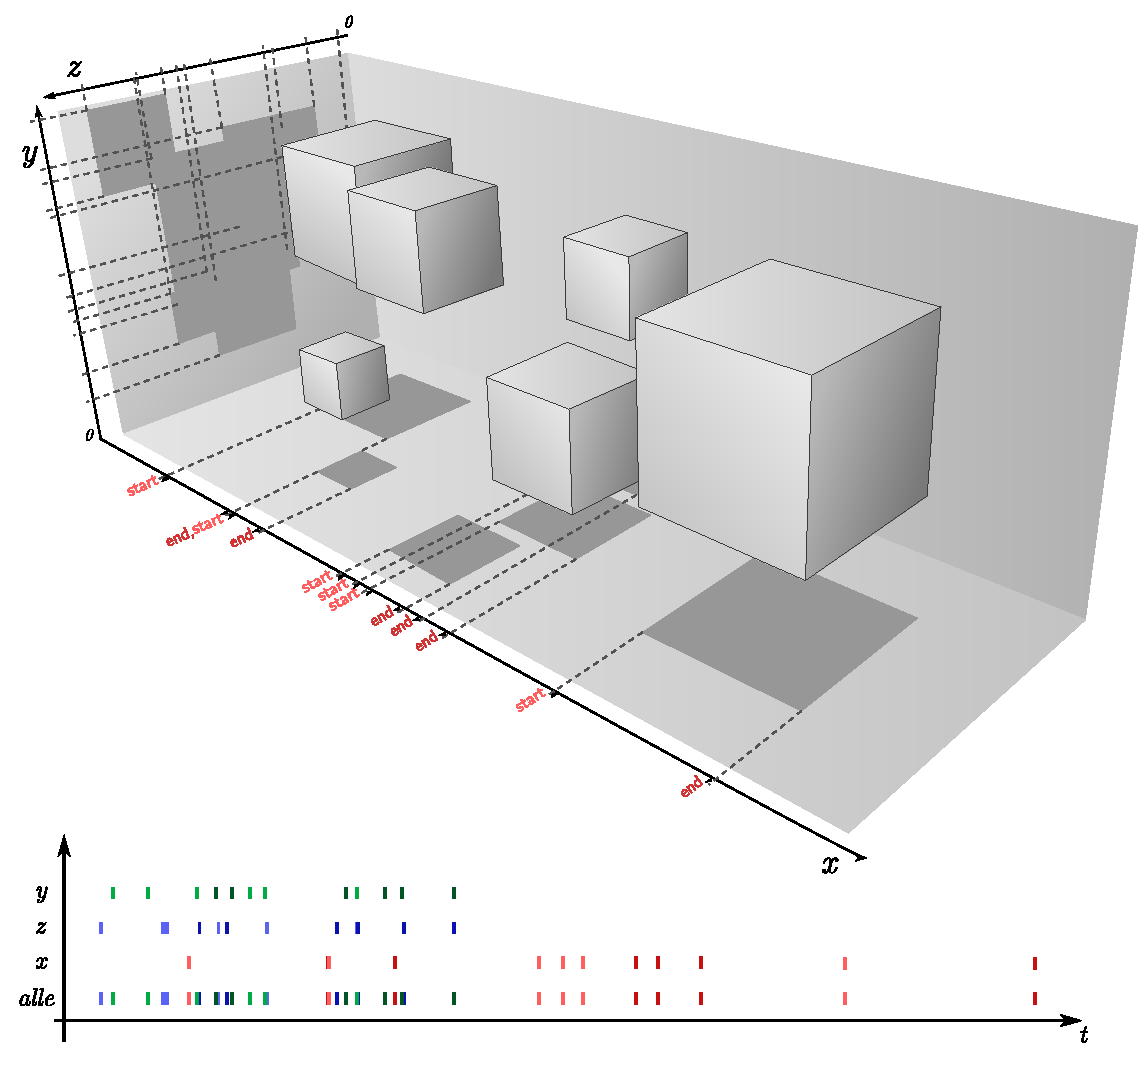
\includegraphics[width=1.0\textwidth]{images/sahnlogn.pdf} 
\caption[Zusammenfassung der Ereignislisten]{Das Minimum einer AABB wird zu einem START-Ereignis, das Maximum zu einem ENDE-Ereignis. Die Ereignisse aller Achsen werden gemeinsam geschachtelt in einer Liste gespeichert.}
\label{fig:eventlist}
\end{figure}

Der so angepasste Algorithmus funktioniert aber nur, wenn er als Eingabe eine bereits (aufsteigend) sortierte Liste aller Ereignisse für den aktuellen Voxel erhält. Damit die Liste für zwei neue Subvoxel nicht aus den Objekten neu erstellt und sortieren werden muss, wird die Ereignisliste des aktuellen Voxels als Grundlage verwendet.
Nachdem die Trennposition $split$ gefunden wurde, muss zunächst für jedes Objekt festgestellt werden, welchen der Subvoxel es überlappt (gegebenenfalls beide). Dazu wird zunächst für alle Objekte konservativ angenommen, dass sie beide Voxel schneiden. Durch Iteration über die Ereignisliste lassen sich die Objekte leicht klassifizieren. Für ``START''-Ereignisse die nach oder in der Trennungsebene liegen kann das zugehörige Objekt als ausschließlich im rechten Voxel liegend markiert werden. Für ``Ende''-Ereignisse, die vor oder in der Trennungsebene liegen, wird das entsprechende Objekt als ausschließlich im linken Voxel liegend markiert. Objekte planarer Ereignisse werden ebenfalls, je nachdem ob sie vor oder hinter der Trennebene liegen, ausschließlich für den linken oder rechten Teilbaum markiert. Für plane Objekte deren Ereignis entlang der Trennachse in der Trennebene liegt, wird das bereits vorgestellte Kriterium, ob einer der beiden Voxel gar keine Objekte enthält angewandt.
In einer weiteren Iteration über die Ereignisse werden nun zwei Teillisten erstellt - eine für den linken und einen für den rechten Voxel. Dabei werden zunächst lediglich die Ereignisse aus der Gesamtliste in die entsprechende Teilliste übernommen, deren Objekte als vollständig im linken oder rechten Voxel liegend markiert wurden.
Objekte, die von der Trennebene geschnitten werden, tragen unterschiedliche Ereignisse zu den beiden Listen bei. Es werden nicht nur die bestehenenden Ereignisse dieser Objekte aufgeteilt sondern auch neue Ereignisse erzeugt. Dies ist notwendig, da das Objekt in beiden Voxeln ``beginnen'' und ``enden'' muss. Die überlappenden Objekte werden hierfür an den Subvoxeln geklippt. Die Minima und Maxima der geklippten Teilobjekte erzeugen die neuen Ereignisse für die jeweilige Teilliste (siehe Abbildung \ref{fig:newevents}). Die neu erzeugten Ereignisse werden für den linken und rechten Teilbaum in einer eigenen Liste gespeichert. Diese verhältnismäßig kurzen Listen lassen sich schnell sortieren. \cite{WaldHavran06} gehen davon aus, dass lediglich $O(\sqrt{N})$ Objekte die Trennebene überlappen. Die Ereignisse hierfür lassen sich demnach in $O(N)$ sortieren.
Danach müssen für beide Teilbäume die Liste der ``alten'' mit der Liste der ``neuen'' Ereignisse zusammengeführt werden. Da beide Listen sortiert sind, lässt sich auch dies in $O(N)$ umsetzen.
\srcref{accelleration}{KdTreeSahNlogN}{construct}

\begin{figure}\centering
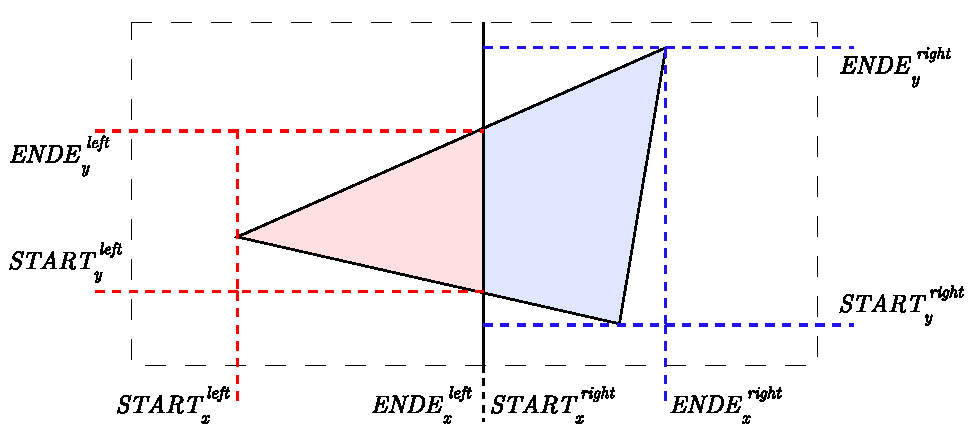
\includegraphics[width=0.6\textwidth]{images/newevents.pdf} 
\caption[Von der Trennebene geschnittenes Dreieck erzeugt neue Ereignisse]{Ein Dreieck welches von der Trennebene geschnitten wird erzeugt Ereignisse in beiden Subvoxeln.}
\label{fig:newevents}
\end{figure}

Der von \cite{WaldHavran06} entwickelte Algorithmus besitzt die algorithmisch niedrigste Komplexität aller bekannten Algorithmen zur Konstruktion kompletter SAH basierter Hierarchien. Er eignet sich allerdings nicht für ``lazy builds'', da der Sortiervorgang am Anfang alle Objekte berücksichtigt.

\subsubsection{Sampling SAH}

Um die Kosten für die Konstruktion weiter zu senken, kann die SAH Auswertung an weniger Stellen vorgenommen werden.
\cite{HWS06} schlagen vor die Anzahl der Primitive zur Linken und zur Rechten der Trennebene an $q$ Positionen auszuwerten. Weitere $q$ Samples werden in den Bereichen ausgewertet in denen die Differenz dieser Werte am größten ist. Durch lineare Interpolation der Objektanzahlen ergibt sich eine stückweise quadratische Kostenfunktion. Das Minimum dieser Funktion wird dann als Position für die Schnittebene gewählt.

Alternativ präsentieren \cite{PGSS06} ein Verfahren, das die Kostenfunktion linear, dafür aber mit 1024 Samples abtastet. Durch die hohe Anzahl der Samples wird eine Verschlechterung der Qualität des konstruierten Baumes weitesgehend vermieden. Das Hauptziel des Verfahrens ist es jedoch, den zufällig verteilten Speicherzugriff anderer Konstruktionssverfahren zu vermeiden. Mehr zur Optimierung von Speicherzugriffen wird in Kapitel \ref{chap:Hardware} erläutert.

\subsubsection{Globale Heuristiken}

Unter globalen Heuristiken versteht man solche, die zur Partitionierung die Szenengeometrie nicht analysieren. Die klassischen Vertreter dieser Kategorie sind der Median der Objektliste und der Median der Szenen-AABB entlang der längsten Achse. Da hier keine Operationen auf den in einem Knoten enthaltenen Objekten ausgeführt werden müssen, lassen sich hiermit Objekthierarchien schneller als mit jedem SAH Verfahren konstruieren.
Der Nachteil dieser Heuristiken ist, dass die resultierenden Hierarchien sich nicht so gut an die lokale Ausprägung der Geometrie anpassen. Strahlanfragen können deswegen meist nicht so effizient beantwortet werden, wie von Datenstrukturen, die mit der SAH konstruiert wurden. Für Anwendungen in denen die Beschleunigungsdatenstruktur jedes Frame neu konstruiert werden muss, kann die Kombination einer ``schnelleren, globalen Konstruktion'' mit einer ``langsameren'' Traversierung unter Umständen den effizienteren Kompromiss darstellen. Gerade bei dynamischen Szenen mit extrem vielen Objekten profitiert die Gesamtleistung von einer sehr schnellen Konstruktion (\cite{BIH06}). Im Gegenzug kann sich eine langsamere Konstruktion in einer Situation in der extrem viele Strahlen ausgesendet werden (z.B. durch hohe Auflösung) durch eine schnelle Traversierungsphase amortisieren.

\section{Zusammenfassung}

Die Anforderung, dynamische Szenen darzustellen, macht die Beantwortung der Frage nach dem \textit{besten} Verfahren nahezu unbeantwortbar. Die bereits totgesagten Verfahren der Partitionierung der Objektmenge erfreuen sich neuer Beliebtheit, dank ihrer Fähigkeit sich veränderten Objektpositionen anzupassen ohne die Topologie neu aufbauen zu müssen.
Auch die Wahl der Heuristik zur Konstruktion ist nicht allgemein zu beantworten. Zu viele Faktoren beeinflussen die Gesamtleistung eines Raytracers. Szenengröße, Auflösung des zu rendernden Bildes, relative Objektgröße und nicht zuletzt die Art in der die Szene spezifiziert wird (z.B. Szenegraph oder ``Suppe'' von Dreiecken) haben großen Einfluss auf die Effizienz der beschriebenen Verfahren.
Aus diesem Grund analysieren viele Verfahren nur den Fall indem die Szene durch eine ungeordnete Menge von Dreiecken - die so genannte \textit{Triangle Soup} - jedes Frame neu spezifiziert wird. Solche allgemeinen Lösungen werden jedoch immer von, für einen Spezialfall angepassten Lösungen, übertroffen werden. So nutzten beispielsweise \cite{RAZOR07} einen durch die Anwendung zu spezifizierenden Szenengraphen um schnell effiziente kd-Trees zu konstruieren.